%\documentclass{llncs}
\documentclass{sig-alternate}
\usepackage{amsmath}
\usepackage{graphicx}
%\usepackage{url}
\usepackage{epic,url}
\usepackage{latexsym}
\usepackage{eepic}
\usepackage{epsfig}
\usepackage{listings}
\usepackage[utf8]{inputenc}
\makeatletter
\newif\if@restonecol
\makeatother
\let\algorithm\relax
\let\endalgorithm\relax
\usepackage[ruled,vlined]{algorithm2e}
\usepackage{amssymb}
\usepackage{rotating}
\usepackage{color}

\usepackage{subfig}
 \makeatletter
 \let\@copyrightspace\relax
 \makeatother

\definecolor{olivegreen}{rgb}{0.2,0.8,0.5}
\definecolor{grey}{rgb}{0.5,0.5,0.5}
\lstdefinelanguage{ttl}{
sensitive=true,
morecomment=[l][\color{grey}]{@},
morecomment=[l][\color{olivegreen}]{\#},
morestring=[b][\color{blue}]\",
}

%\usepackage[top=4cm, bottom=4cm, left=4.5cm, right=4.5cm]{geometry}
%\renewcommand{\baselinestretch}{0.990}


\sloppy

\newtheorem{definition}{Definition}
\newtheorem{example}{Example}
%\newtheorem{proposition}{Proposition}
\newtheorem{theorem}{Theorem}
\newtheorem{lemma}{Lemma}
%\newtheorem{property}{Property}
\newtheorem{myproof}{Proof}
\newtheorem{goal}{Goal}

\newcommand{\dtr}[1]{(\textbf{dtr: #1})}
\newcommand{\sem}[1]{\mbox{ $[\![ #1 ]\!]$}}
\newcommand{\gla}[1]{(\textbf{gla: #1})}
\newcommand{\todo}[1]{(\textbf{TODO: #1})}


\title{Multi-objective Linked Data Query Optimization}

\numberofauthors{2}
\author{
  % \alignauthor
  % Günter Ladwig \\
  % \affaddr{Institute AIFB} \\
  % \affaddr{Karlsruhe Institute of Technology, Germany} \\
  % \affaddr{D-76128 Karlsruhe} \\
  % \email{guenter.ladwig@kit.edu}
  % \alignauthor
  % Thanh Tran \\
  % \affaddr{Institute AIFB} \\
  % \affaddr{Karlsruhe Institute of Technology, Germany} \\
  % \affaddr{D-76128 Karlsruhe} \\
  % \email{ducthanh.tran@kit.edu}
}

% \author{Günter Ladwig, Thanh Tran}
% \authorrunning{Ladwig et al.}
% \institute{
% Institute AIFB, Karlsruhe Institute of Technology, Germany\\
% \email{\{guenter.ladwig,ducthanh.tran\}@kit.edu}
% }

\setlength{\algomargin}{0.4cm}
\SetAlgoSkip{}

\begin{document}
\maketitle
\begin{abstract} 
  With the proliferation of the Web of data and Linked Data in
  general, approaches for processing queries directly over remote
  Linked Data have recently gained attention. These approaches address
  new challenges such as the large amount of data sources and the
  highly distributed nature of Linked Data. However, all approaches
  have in common that, for a variety of reasons, they are usually not
  able to answer queries completely. We argue that completeness is no
  longer a requirement when processing queries over Linked Data and
  observe an inherit trade-off between completeness and execution
  cost. We propose to employ multi-objective optimization in order to
  simultaneously optimize for the conflicting objectives completeness
  and cost. In order to achieve this, we integrate source selection
  into the query optimization process, define a cost model for Linked
  Data query plans and adapt the traditional dynamic programming
  algorithm for query optimization to perform \emph{multi-objective
    query optimization}. 

\end{abstract}

\section{Introduction}
\label{sec:linked_data} 

In recent years, the amount of Linked Data on the Web has been
increasing rapidly. This is largely due to community efforts such as
the Linking Open Data project, and increasing interests of enterprises
and governments. Datasets made publicly available on the Web as Linked
Data cover different domains, including life sciences (e.g. DrugBank,
UniProt, PubMed), geographic locations (e.g. World Factbook, Geo Names), media and entertainment (MusicBrainz, Last.FM, BBC
Programmes). There are also cross-domain encyclopedic datasets such as
Freebase and DBpedia (the structured data counterpart of
Wikipedia). Besides enterprises, such as media companies like BBC and
Last.FM, many governments (e.g. US, UK) recently started to make data
of public interest available to citizens, including CO2, Mortality,
Energy and Postcodes. We refer to the public
Website~\footnote{\url{http://linkeddata.org/}} for an overview of
concepts, activities, projects, and datasets related to Linked Data.

Aiming at making Linked Data available to
data-intensive processes and Web users, researchers recently started
to study the problem of Linked Data query
processing~\cite{hartig_executing_2009,harth_data_2010,ladwig_linked_2010,hartig_zero_2011,sihjoin_2011}. Just
like Web pages, Linked Data on the Web are accessible through URI
lookups. According to the Linked Data principles
\cite{bizer_linked_2009}, dereferencing a Linked Data URI via HTTP
should return a machine-readable description (usually in RDF) of the
entity identified by the URI. Each URI therefore represents a virtual
``data source''.

Figs.~\ref{fig:sources} \& \ref{fig:query} show examples of Linked
Data sources with their data and a Linked Data query,
respectively. For processing such a query, Linked Data sources to be used may not be stored or cached locally, but
are retrieved at run-time via dereferencing the URIs mentioned in the sources. In this way,
Linked Data query processing specifically aims to deal with the rapidly evolving nature of
the Web of data and to deliver results that are always
up-to-date. In this example, the query engine may dereference the
URIs \emph{ex:beatles}, \emph{ex:sgt\_pepper} and \emph{ex:lucy} to
produce the result \emph{``Lucy...''} for the query variable
$?name$.
% \dtr{need example which illustrate what is linked
%   data query processing, and why it is really useful, e.g. freshness
%   of results important due fast update rates of data, what else?}

Thus, processing structured queries against Linked Data can be seen as
a special case of federated query processing. However, the restricted
access pattern based on HTTP lookup and the highly distributed nature
of Linked Data sources resulting from it, present unique challenges:

\begin{figure*}[ht]
  \centering
  \begin{minipage}{0.32\linewidth}
\begin{lstlisting}[breaklines=true,language=ttl,linewidth=0.98\linewidth,frame=single,caption=http://example.org/beatles]
ex:beatles 
  foaf:name "The Beatles" ;
  ex:album ex:help ;
  ex:album ex:sgt_pepper  .
\end{lstlisting}
    \vspace{-0.4cm}
  \end{minipage}
  \begin{minipage}{0.32\linewidth}
\begin{lstlisting}[breaklines=true,language=ttl,linewidth=0.98\linewidth,frame=single,caption=http://example.org/help]
ex:help 
  foaf:name "Help!" ;
  ex:song ex:night ;
  ex:song ex:girl .
\end{lstlisting}
    \vspace{-0.4cm}
  \end{minipage}
  \begin{minipage}{0.32\linewidth}
\begin{lstlisting}[breaklines=true,language=ttl,linewidth=0.98\linewidth,frame=single,caption=http://example.org/sgt\_pepper]
ex:sgt_pepper
  foaf:name "Sgt. Pepper" ;
  ex:song ex:lucy ;
  ex:song ex:friends .
\end{lstlisting}
    \vspace{-0.4cm}
  \end{minipage}
  \begin{minipage}{0.32\linewidth}
\begin{lstlisting}[breaklines=false,language=ttl,frame=single,linewidth=0.98\linewidth,caption=http://example.org/girl]
ex:girl
  foaf:name "Another Girl" .

\end{lstlisting}
  \label{fig:example}
  \end{minipage}
  \begin{minipage}{0.32\linewidth}
\begin{lstlisting}[breaklines=true,language=ttl,frame=single,linewidth=0.98\linewidth,showlines=true,caption=http://example.org/night]
ex:night 
  foaf:name "The Night..." .
\end{lstlisting}
  \end{minipage}
  \begin{minipage}{0.32\linewidth}
\begin{lstlisting}[breaklines=true,language=ttl,frame=single,showlines=true,caption=http://example.org/lucy]
ex:lucy
  foaf:name "Lucy..." .
\end{lstlisting}
  \end{minipage}

\vspace{-0.3cm}
  \caption{Example Linked Data sources. The prefix \emph{ex:} expands
    to ``http://example.org/''.}
  \label{fig:sources}
\vspace{-0.3cm}
\end{figure*}

\begin{itemize}
\item \textbf{Large number of sources.} Since every URI can be
  considered as a source, the \emph{number of Linked Data sources}
  that have to be processed is potentially very large. Hundreds of
  sources of varying size may have to be retrieved for a single
  trivial query~\cite{ladwig_linked_2010}.

\item \textbf{High cost for source retrieval.} Typically, while basic
  source statistics have been assumed to exist (especially for sources
  that have been processed before~\cite{ladwig_linked_2010}), it is
  not practical or desirable to assume that all data is available
  locally. Processing queries in
  this distributed setting however requires Linked Data sources to be
  \emph{retrieved as a whole}. This is because as opposed to standard
  federated query processing, where remote sources are actually
  endpoints that provide structured querying capabilities, only HTTP
  lookups are possible here. That is, instead of retrieving partial
  answers that possibly match large parts of the queries, only whole
  sources matching the URIs mentioned in the queries can be
  obtained. As a result, processing Linked Data sources becomes a
  separate task, and due to its relative high cost, requires special
  treatment during query processing.
  %	Without these advanced querying capabilities, the impact of
  % selecting sources on overall query performance becomes more
  % pronounced as the overhead of source retrieval is much higher.

\item \textbf{Different, conflicting optimization criteria.}
  Typically, the optimization of queries is based on one single goal,
  namely to minimize the \emph{cost} for computing all results. The
  large number of potentially relevant sources and their high
  processing costs lead to long execution times such that \emph{result
    completeness} is often no longer affordable in practical
  usage. Thus, addressing this requirement has not been the main goal in
  previous work on Linked Data query
  processing~\cite{hartig_executing_2009,harth_data_2010,ladwig_linked_2010}, which
  employs various termination criteria such as a maximum number of
  retrieved sources \cite{harth_data_2010}, and strategies to select only the best few sources~\cite{ladwig_linked_2010}. 
%  In 
%  fact, completeness has
%  never been crucial on the Web but rather, the goal of Web search for
%  instance, is to obtain some (best) results in a given amount of
%  time. In other words, not only the cost of processing but also the
%  amount of results (\emph{output cardinality}) play a role. 
  Instead of assuming completeness and optimizing exclusively for cost, other 
  criteria such as relevance, quality and cardinality of results, and trustworthy of sources may be considered in the various Linked Data use cases that are
  possible. This is problematic because these criteria are not always
  complementary. For instance, there is an inherent trade-off between
  output cardinality and cost: To produce more results, we have to
  retrieve more sources, which in turn increases processing cost (and
  vice versa).
\end{itemize}

\emph{Federated databases} are able to process queries over data that
is managed by several networked database systems, either centralized
\cite{zsu_principles_2011} or in a distributed, peer-to-peer fashion
\cite{huebsch_architecture_2005}. Every node in this federated setting 
hosts its data, and provides structured querying
capabilities such that query processing in this setting breaks down to
finding the right nodes to execute part of the queries and merging
results. For optimization, the main strategy is to leverage the
capabilities of the nodes, i.e. pushing the processing to the nodes,
and to minimize cost for transferring data (partial results)
\cite{kossmann_iterative_2000,zsu_principles_2011}. In the case where
nodes provide materialized views, this problem amounts to finding the
cost-optimal composition of views
\cite{pottinger_minicon:_2001}. These solutions are not applicable to
our setting because instead of partial results and views, nodes return
entire sources. That is, they possess only one capability, namely
``source scan'' (we choose this term to make clear the analogy of HTTP
source lookup and table scan). More precisely, \emph{not the
  composition of views or joined results but the selection of source scans and processing the resulting sources are crucial tasks in this setting.}
%Standard query optimization can be adopted to produce an optimal query plan. 

% Further, as completeness is not required, not only the order but also
% the selection of sources is critical for query optimization.
Selecting relevant sources for a given query has been a topic in
data integration research. There, sources are described
not only by their content, but also by their capabilities, and
algorithms that efficiently perform \emph{source selection} by using
source characteristics to prune the search space have been
proposed~\cite{levy_querying_1996}. However, source selection is
performed as a separate step. Also decoupled from query optimization
are the source ranking strategies recently applied in Linked Data
query processing~\cite{harth_data_2010,ladwig_linked_2010}. Because
source selection is an essential part of query processing, this kind
of \emph{local optimization may lead to sub-optimal overall plans}.
%\cite{nie_joint_2001}.


Further, all these approaches \emph{optimize towards one single
  criterion} (cost) only.

\begin{figure}[ht]
  \vspace{-0.3cm}
  \centering
  \begin{minipage}{0.75\linewidth}
\begin{lstlisting}[language=ttl,numbers=left,escapeinside={(*@}{@*)}]
SELECT ?name WHERE {
  ex:beatles ex:album  ?album . (*@\label{query:q1}@*)
  ?album     ex:song   ?song . (*@\label{query:q2}@*)
  ?song      foaf:name ?name . (*@\label{query:q3}@*)
}
\end{lstlisting}
  \vspace{-0.3cm}
  \end{minipage}
  \vspace{-0.3cm}
  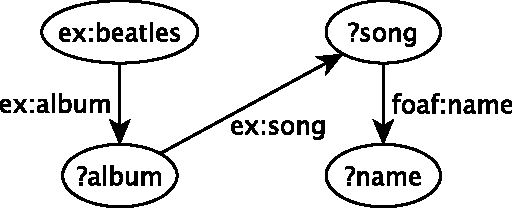
\includegraphics[width=0.7\linewidth]{figs/query-crop.pdf}
  \caption{Example query asking for names of songs in albums of the
    Beatles. The query consists of three triple patterns $t_1$ (line
    \ref{query:q1}), $t_2$ (line \ref{query:q2}), and $t_3$ (line
    \ref{query:q3}).}
  \label{fig:query}
\end{figure}

\textbf{Contributions.} Aiming at the challenges presented above, we
provide the following contributions:

\begin{itemize}
\item Solutions related to Linked Data query processing include Linked
  Data indexing~\cite{harth_data_2010}, query processing
  strategies~\cite{hartig_executing_2009,ladwig_linked_2010}, and
  using heuristics for adaptive ranking to select only the few best
  sources~\cite{ladwig_linked_2010}. However, to the best of our
  knowledge, this work is the \emph{first solution towards a
    systematic optimization of Linked Data query processing}.

\item In particular, we propose an optimization framework for Linked Data query processing, which incorporates
  \emph{both standard query operators} and \emph{source
    selection}. That is, we propose to extend the scope of query
  optimization from how to process data to which data to process. This
  is necessary to reflect the nature of Linked Data query processing,
  where source selection and scanning become an essential
  part. Further, this framework supports the \emph{joint optimization
    of several objectives}, cost and output cardinality in particular.

\item We propose a dynamic programming algorithm for the
  multi-objective optimization of this integrated process of source
  selection and query processing. It produces a set of Pareto-optimal
  query plans, which represent different trade-offs between optimization
  objectives.
  
\item After retrieval, sources can be re-used in different parts of
  the query. Essentially, this means that \emph{sharing of source
    scan operators} is possible. While this provides more room for
  optimization, it also makes dynamic programming technically more
  challenging: the cost function is no longer monotonic with regard to
  plan combination, which is due to the fact that the cost of subplans
  may vary, depending on the reusability of their sources. We provide
  \emph{tight bounds} for costs that take this effect into account.
\end{itemize}



% In this paper, we apply multi-objective optimization to the task of
% optimizing Linked Data queries. As shown in previous work
% \cite{harth_data_2010,ladwig_linked_2010} source selection and ranking
% are integral tasks of executing queries over Linked Data. We therefore
% propose to extend the scope of query optimization from choosing
% \emph{how} to process data to also decide \emph{which} data to process
% by integrating source selection and ranking into the query
% optimization process. \todo{also necessary because we want to optimize
%   both objectives...}

\textbf{Outline.} In Section~\ref{sec:problem} we introduce the
problem of multi-objective Linked Data query processing. In
Section~\ref{sec:framework} propose an optimization framework for
Linked Data query processing. Section~\ref{sec:opt} describes our
adaptation of the dynamic programming query optimization algorithm for
multi-objective query optimization.  Section~\ref{sec:related} gives
and overview of related work. Finally, we evaluate our approach in
Section~\ref{sec:eva} before concluding in
Section~\ref{sec:conclusion}.




%%% Local Variables: 
%%% mode: latex
%%% TeX-master: "paper"
%%% End: 

\section{Problem Definition}
\label{sec:problem}
We first define the data and query model and then
introduce the problem of processing queries over Linked Data.

\subsection{Linked Data and Queries} 
RDF~\cite{klyne_resource_2004} is used
as the data model, but for clarity of presentation, we do not consider
the special RDF semantics (e.g. RDF blank nodes) and focus on the main characteristic of RDF. 
%However, all methods presented in this paper can easily
%be extended to deal with blank nodes. 
Namely, it can be considered as a general model for
graph-structured data encoded as $\langle subject, predicate, object
\rangle$ triples. These triples are composed of unique identifiers
(URI references) and literals (e.g., strings or other data values) as
follows:

% As usual~\cite{hartig_executing_2009,ladwig_linked_2010}, we
% conceive Linked Data sources as interlinked sets of RDF triples
% \cite{klyne_resource_2004}.

\begin{definition}[RDF Triple, RDF Term, RDF Graph]
  Given a set of URI references $\mathcal{U}$ and a set of literals
  $\mathcal{L}$, elements in $\mathcal{U} \cup
  \mathcal{L}$ are called \emph{RDF terms},
  $\langle s, p, o\rangle \in \mathcal{U}
  \times \mathcal{U} \times (\mathcal{U} \cup \mathcal{L})$ is 
  an \emph{RDF triple}, and every set of RDF triples is also called
  a \emph{RDF graph}.
\end{definition}

It is a graph because RDF triples can be seen 
as edges connecting nodes that stand for RDF terms. URI references in RDF are used to uniquely identify resources captured by the data. 
%(instances, concepts, properties) and allow assertions to be made about their attributes and
%relationships. 
The Linked Data principles \cite{bizer_linked_2009} commonly used on the Web to access and publish RDF data (as Linked Data) mandate
that HTTP URIs shall be used and that dereferencing such an URI returns a
description of the resource identified by the URI. While these principles are also applicable to other types of data, 
the large amount of descriptions published this way on the Web represent RDF graphs, each is a set of triples where the dereferenced URI appears as subject or object.

Therefore, a HTTP URI reference can be seen as a data source, whose
content can be obtained by dereferencing the HTTP URI. Triples in
these \emph{Linked Data sources} contain other HTTP URI
references. Following these URIs lead to other sources. When it is
clear from the context, we will make no distinction between the
resource identified by an URI and the Linked Data source that can be
retrieved by dereferencing that URI.

\begin{definition}[Linked Data Source]
  A \emph{Linked Data source}, identified by an HTTP URI $d$, is a set of RDF triples $\langle s,p,o \rangle$ . Dereferencing an
  HTTP URI $d$ can be seen as a function $deref : \mathcal{U} \rightarrow \mathcal{T}$, which maps a URI to a set of triples such that the set of triples $T^d$ for $d$ can be obtained as $T^d = \mathit{deref}(d)$. There is a \emph{link} between two Linked Data
  sources $d_i, d_j$ if $d_j$ appears as the subject or object in at
  least one triple of $d_i$, i.e. $\exists t\in T^{d_i},t=\langle d_j,p,o \rangle \vee t=\langle s,p,d_j \rangle$ or vice versa, $\exists t\in T^{d_j},t=\langle d_i,p,o \rangle \vee t=\langle s,p,d_i \rangle$. The union set of
  sources $d_i \in D$ constitutes the \emph{Linked Data} graph
  $T^D=\{t| t \in T^{d_i}, d_i \in D\}$.

  % A \emph{source} $d$ is a set of RDF triples $\langle s^d,p^d,o^d
  % \rangle \in T^d$ where $s^d$ is called the subject, $p^d$ the
  % predicate and $o^d$ the object. There is a function $ID$ which
  % associates a source $d$ with a unique URI. There is a \emph{link}
  % between two sources $d_i$ and $d_j$ if the URI of $d_i$ appears as
  % the subject or object in at least one triple of $d_j$, i.e.,
  % $\exists t \in T^{d_j}: s^d(t) = ID(d_i) \vee o^d(t) = ID(d_i)$; or
  % vice versa, i.e., $\exists t \in T^{d_i}: s^d(t) = ID(d_j) \vee
  % o^d(t) = ID(d_j)$ (then $d_i$ and $d_j$ are said to be
  % \emph{interlinked}). The union set of interlinked sources $d_i \in
  % D$ constitutes the \emph{Linked Data} $T^D=\{t| t \in T^{d_i}, d_i
  % \in D\}$.
\end{definition}

The standard language for querying RDF data is SPARQL
\cite{prudhommeaux_sparql_2008}. An important feature of SPARQL 
is basic graph pattern (BGP). Work on RDF and Linked Data query processing
so far focused on the task of answering BGP queries. For ease of notation, we use $t$ both to denote triples and triple patterns: 
%, i.e., queries
%that consist of a single BGP.

\begin{definition}[Triple Pattern, Basic Graph Pattern]
  A \emph{triple pattern} $t=\langle s,p,o \rangle$, where each $s$, $p$ and $o$ is either a RDF term (called \emph{constant}) or a variable. A \emph{basic graph pattern} is a set of triple patterns $Q= \{t_i,\ldots,t_n\}$. 
\end{definition}

Typically, every triple pattern in $Q$ shares one common variable with at least one other pattern in $Q$ such that $Q$ forms a connected graph. Computing answers to a BGP query over the Linked Data graph amounts to the
task of \emph{graph pattern matching}. A result to a BGP query can be defined as
follows:

\begin{definition}[Result]
Let $T^D$ be the Linked Data graph, $TERM$ be the set of RDF terms in $T^D$, $Q$ be a BGP query, and $V$ be the set of all variables in $Q$. Then a mapping
$\mu_{T^D}: V \to TERM$ from the variables in $Q$ to RDF terms
in $T^D$ will be called a \emph{result} to $Q$, if the function
\[
\mu'_{T^D}: V \cup TERM \to TERM \left\{
\begin{array}{ll}
v \mapsto \mu_{T^D}(v) & \mbox{ if } v\in V \\
l \mapsto l & \mbox{ if } l \in TERM\\
\end{array}\right.
\]
satisfies $\langle \mu'_{T^D}(s),\mu'_{T^D}(p), \mu'_{T^D}(o) \rangle \in T^D$ for any $\langle s,p,o \rangle \in Q$. 
\end{definition}

We will use $\mu_{T^D}$ not only to refer to
the result nodes in ${T^D}$ that match the query variables but also the
triples (subgraphs) that match a triple pattern (a BGP).
% Since Linked Data triples in $T^D$ also form a graph, processing
% queries in this context amounts to the task of graph pattern
% matching. In particular, an \emph{answer} (also called a \emph{query
% binding}) to a BGP query is given by $\mu$ which maps the query
% graph pattern $T^q$ to subgraphs $T^D_q \in T^D$. By applying such a
% mapping, each variable in $T^q$ is replaced by the corresponding
% subject, predicate or object of the matching triples in $T^D$. The
% mapping of a triple pattern $t^q \in T^q$ to triples $T^D_{t^q}
% \subseteq T^D$ are called \emph{triple bindings}; and $T^D_{t^q}(v)$
% denotes the set of matches found for the variable $v$ of $t^q$
% called \emph{variable bindings}.

%In the context of Linked Data query processing, the RDF graph over
%which queries are executed is the Linked Data graph $T^D$, the union
%set of all Linked Data sources $d \in D$. 

\subsection{Processing Linked Data Queries} A BGP query is evaluated by
first obtaining bindings for each of its constituent triple patterns $q
\in Q$ and then performing a series of joins between the bindings. This is done for every two patterns that share a
variable, forming a \emph{join pattern} (that variable is referred to
as the \emph{join variable}). 
%For most queries there are multiple ways to obtain results, e.g.,
%joins can be executed in different orders or different methods might
%be used to access input data. Some ways might be more efficient than
%others. It is the task of the \emph{query optimizer} to find an
In the Linked Data context, BGP queries are 
%not
%%evaluated on a single source, but, in order to obtain all results,
%%they have to be matched against the combined graph 
evaluated against the set of all sources in the Linked Data graph $T^D$. 
While some sources may be available locally, others have
to be \emph{retrieved via HTTP dereferencing during query processing}. 

Previous work on Linked Data query processing
%, two main approaches
%to discover sources were described. 
implements exploration-based \emph{link traversal} 
%  does not rely on having complete knowledge about all
%Linked Data sources
\cite{hartig_executing_2009,hartig_zero_2011}. 
%These approaches take
%advantage of links between sources and discover new sources at
%run-time by traversing these links. 
%In \cite{hartig_executing_2009},
%no knowledge is available at all, and 
For this, the query is assumed to contain at least one constant that is a URI. This URI is used for retrieving
the first source, representing the ``entry point'' to Linked Data. Triples in this entry point represent links to other sources. By following these links, new
sources are discovered and retrieved. When retrieved sources contain data matching the query triple patterns, they are selected and joined to produce query results. 

Knowledge about (previously processed) Linked Data sources in the form of statistics has been exploited 
%to 
%assumes that all source descriptions are available and based on that,
%compiles a query evaluation plan that specifies 
to determine and rank relevant sources~\cite{harth_data_2010}. 
%and the order for retrieving and processing these sources. Source
%discovery and query optimization is an offline process and no new
%sources are discovered at run-time.
The authors of that work~\cite{harth_data_2010} focus on the efficient encoding and processing of these statistics. Instead of ranking sources at compile time, adaptive re-ranking of sources at runtime has also been proposed~\cite{ladwig_linked_2010}. Common statistics used for processing Linked Data sources include a \emph{source index}:


\begin{definition}[Source Index]
  \label{def:index}
  Given the Linked Data sources $D$, the \emph{source index} can be conceived as a function $source : \mathcal{T} \to 2^\mathcal{URI}$, which maps a triple pattern $t$ to URIs representing sources that contain results for $t$, i.e. $source(t) =
  \{d| d \in D \wedge, \mu_{T^d}(t) \neq \emptyset \}$. 
\end{definition}
%
%\begin{definition}
%  source description, statistics
%\end{definition}

In practice, the source index used by existing work not only returns the URIs but also basic source descriptions that provide selectivity information for triple and join patterns. For instance, these statistics are stored for previously discovered sources, or collected from catalogs of Linked Data sources such as CKAN\footnote{\url{http://ckan.net}}.
%As mentioned before, there are sourcces previous work, additional knowledge about sources captured by the VoiD vocabulary (common standard\footnote{\url{http://semanticweb.org/wiki/VoiD }} used to describe interlinked datasets) and   
%Given a query, we use the source index to
%discover all relevant known sources, i.e., all sources that contain
%triples matching query triple patterns. While there might be relevant
%sources that are not discovered because they are not part of the
%source index, query processing can be complete with regard to the data
%in sources indexed by the source index.

Given the large number of Linked Data sources and their high retrieval costs, it is often not practical to process all relevant sources. The heavily skewed data
distribution of Linked Data exacerbates this problem, as there are
triple patterns that match all or many sources and therefore do not
help to discriminate sources \cite{ladwig_linked_2010}. For example, 
the pattern $\langle ?x, \mbox{\emph{rdf:type}}, ?y \rangle$ matches most Linked Data sources. Thus, existing work rank and process only a few sources~\cite{harth_data_2010,ladwig_linked_2010}.

%\subsection{Pareto Optimal Linked Data Query Optimization} 
%While these existing ad-hoc strategies for processing Linked Data sources can improve performance, there exists no query optimization technique that compute and guarantee the optimality of query plans. We provide the first attempt towards Linked Data query optimization, 


\section{Linked Data Query Optimization Framework}
\label{sec:framework}
These existing ad-hoc strategies for selecting Linked Data sources have shown to improve the performance of Linked Data query processing. However, there exists no optimization technique that goes beyond source selection to consider the entire process of Linked Data querying. In this section, we provide a systematic study of existing Linked Data querying approaches~\cite{hartig_executing_2009,harth_data_2010,ladwig_linked_2010} to model the querying process in terms of operators of a query plan. The goal is to provide the first \emph{systematic solution towards Linked Data query optimization}, which considers the effect of query operators to compute and guarantee the optimality of query plans. 

%For optimizing Linked Data queries, we systematically captures all operators needed, incorporate them into a query plan, and briefly, discuss how to estimate their impacts on the optimization objectives cost and outputs. 

\subsection{Query Operators}
\label{sec:ops}
%For processing linked data queries, sources containing data for query triple patterns have to be retrieved (possibly from remote sources). We use a \emph{source scan} operator to represent sources. Then, standard query operators are adopted to process triples retrieved from these sources.
%Triples in the same source however, can be used to answer different patterns. Selecting triples from sources is captured by the \emph{selection} operator. Triples for a pattern retrieved from all sources are then combined via the \emph{union} operator, and finally, combined with triples retrieved for other patterns via \emph{join}: 
% when these patterns share a common variable, via union otherwise. 
The standard query operators table scan, selection, union and join can be used to model the Linked Data querying process. The main difference to traditional query processing is that the availability of data indexes cannot be assumed in the general case. Only some basic statistics about sources can be assumed to available such that given a triple pattern, relevant sources can be determined~\cite{harth_data_2010,ladwig_linked_2010}. However, entire sources have to be retrieved. This is conceptually same to table scans. The difference is that often, sources have to be retrieved from remote sites via HTTP URI lookup. Moreover, several sources may contain answers for one single query predicate (triple pattern in this case).  

\begin{definition}[Source Scan] The input of a source scan operator $scan(d)$ is the source URI $d$.
% consists of the data contained in
%such a source. 
Executing this operator outputs all triples in $d$, i.e. $scan(d) = T^d$.
\end{definition}

\begin{definition}[Selection]  A selection $\sigma_t(T^d)$ is performed on the input $T^d$ to output
triples in $T^d$ that match $t$, i.e. $\sigma_t(T^d) = \mu_{T^d}(t)$. 
\end{definition}

Outputs from two triple patterns $t_i$ and $t_j$ that share a common variable are combined through a standard join operator $\mu(t_i)\Join\mu(t_j)$. 

\begin{definition}[Union] As usual, $\bigcup(I_1,\ldots,I_n)$
outputs the union of its inputs $I_i$, $1\leq i < \leq n$, where every input $I_i$ stands for results for one triple pattern, $I_i = \mu_{T^d}(t)$, or several triple patterns, e.g. $I_i = \mu_{T^d}(t_i)\Join\mu_{T^d}(t_j)$. Because a triple pattern can match several sources, $I_i$ may also capture partial results for a pattern $t$ such that the union
$\bigcup(\sigma_t(T^{d_1}),\ldots,\sigma_t(T^{d_n}))$ combines results from several selection operators.   
\end{definition}

For clarity of presentation, we assume query triple patterns form a connected graph such that join is the only operator used to combine triples from different patterns. 


\subsection{Query Plan}
\label{sec:basicshape}
Query plans for relational databases generally consist of access plans
for individual relations whose outputs are then processed by join and
other operators. We take a similar approach and create an
access plan for each triple pattern, which consists of source scan, selection and union
operators:

\begin{definition}[Access Plan]
  Given a query $Q$, let $t \in Q$ be a triple pattern in $Q$ and $D = source(t)$ be the set of sources for $t$. An access plan $p(t)$ for $t$ is a tree-structured query plan constructed in the
  following way:
  \begin{itemize}
  \item At the lowest level, the leaf nodes of $p(t)$ are source scan operators, one
    $scan_t(d_i) = T^{d_i}$ for each $d_i \in D$.
  \item The next level contains selection operators, one
    for processing the output of every scan operator, i.e. we have $\sigma_t(T^{d_i})$ for every $d_i \in D$.     
   \item The root node is a union operator $\bigcup_t(\sigma_t(T^{d_1}),\ldots,\sigma_t(T^{d_{|D|}}))$ that combines the outputs of all selection operators for $t$.    
  \end{itemize}
\end{definition}

At the next levels, the outputs of access plans' root operators are successively
joined to process all triple patterns of the query, resulting in a \emph{tree of operators}. However, in Linked Data query processing, it is often the case that a single
Linked Data source contains data matching several triple patterns. It
is therefore possible that a data source is used for more than one
query triple pattern. In this case it is detrimental to execute the
scan operator more than once as this will incur network costs that can
be avoided. We therefore perform \emph{operator sharing}, where the
output of a source scan operator is used as input for more than one
selection operators, i.e. the output is shared. This means that access plans may
overlap and the overall query plan is no longer a tree, but has the form of a directed
acyclic graph (DAG) \cite{Neumann_2005}. \dtr{discuss how to process such a graph}

%\begin{definition}[Linked Data Query Plan]
%  Given the query $Q=\{t_1,\ldots,t_n\}$ and the corresponding access plans for every triple pattern $A(Q) = \{p(t_i),\ldots,p(t_n)\}$, a \emph{Linked Data query plan} $p(Q)$ for the query $Q$ represents the sequence of joins $\langle Join_1\ldots\Join_n \rangle$ such that 
%\begin{itemize}
%	\item For every join
%\end{itemize}  
%  	
%  for a query $Q$ is a DAG with
%  nodes representing query operators, and edges representing the data
%  flow between operators. A Linked Data query plan is constructed from
%  access plans for single triple patterns for all $q_i \in Q$, whose
%  outputs are then combined using join operators.We use $P(Q)$ and
%  $P^+(Q)$ to denote the set of all query plans and the set of optimal
%  plans, respectively, which produce results for a query $Q$.
%\end{definition}

% At the first level, a Linked Data query plan consists of source scan
% operators, one for each source that has to be processed. Because
% entire sources have to be retrieved, often at very high costs due to
% network latency, selecting the right sources is critical in Linked
% Data query optimization. At the next level, selection operators
% process source data to output triples that match the query triple
% patterns. Selection operators are connected to union operators, which
% combine results for every query triple pattern. There is one union
% operator for every triple pattern. They act as base inputs for the
% join operators.

\begin{figure}[htb]
  \centering
  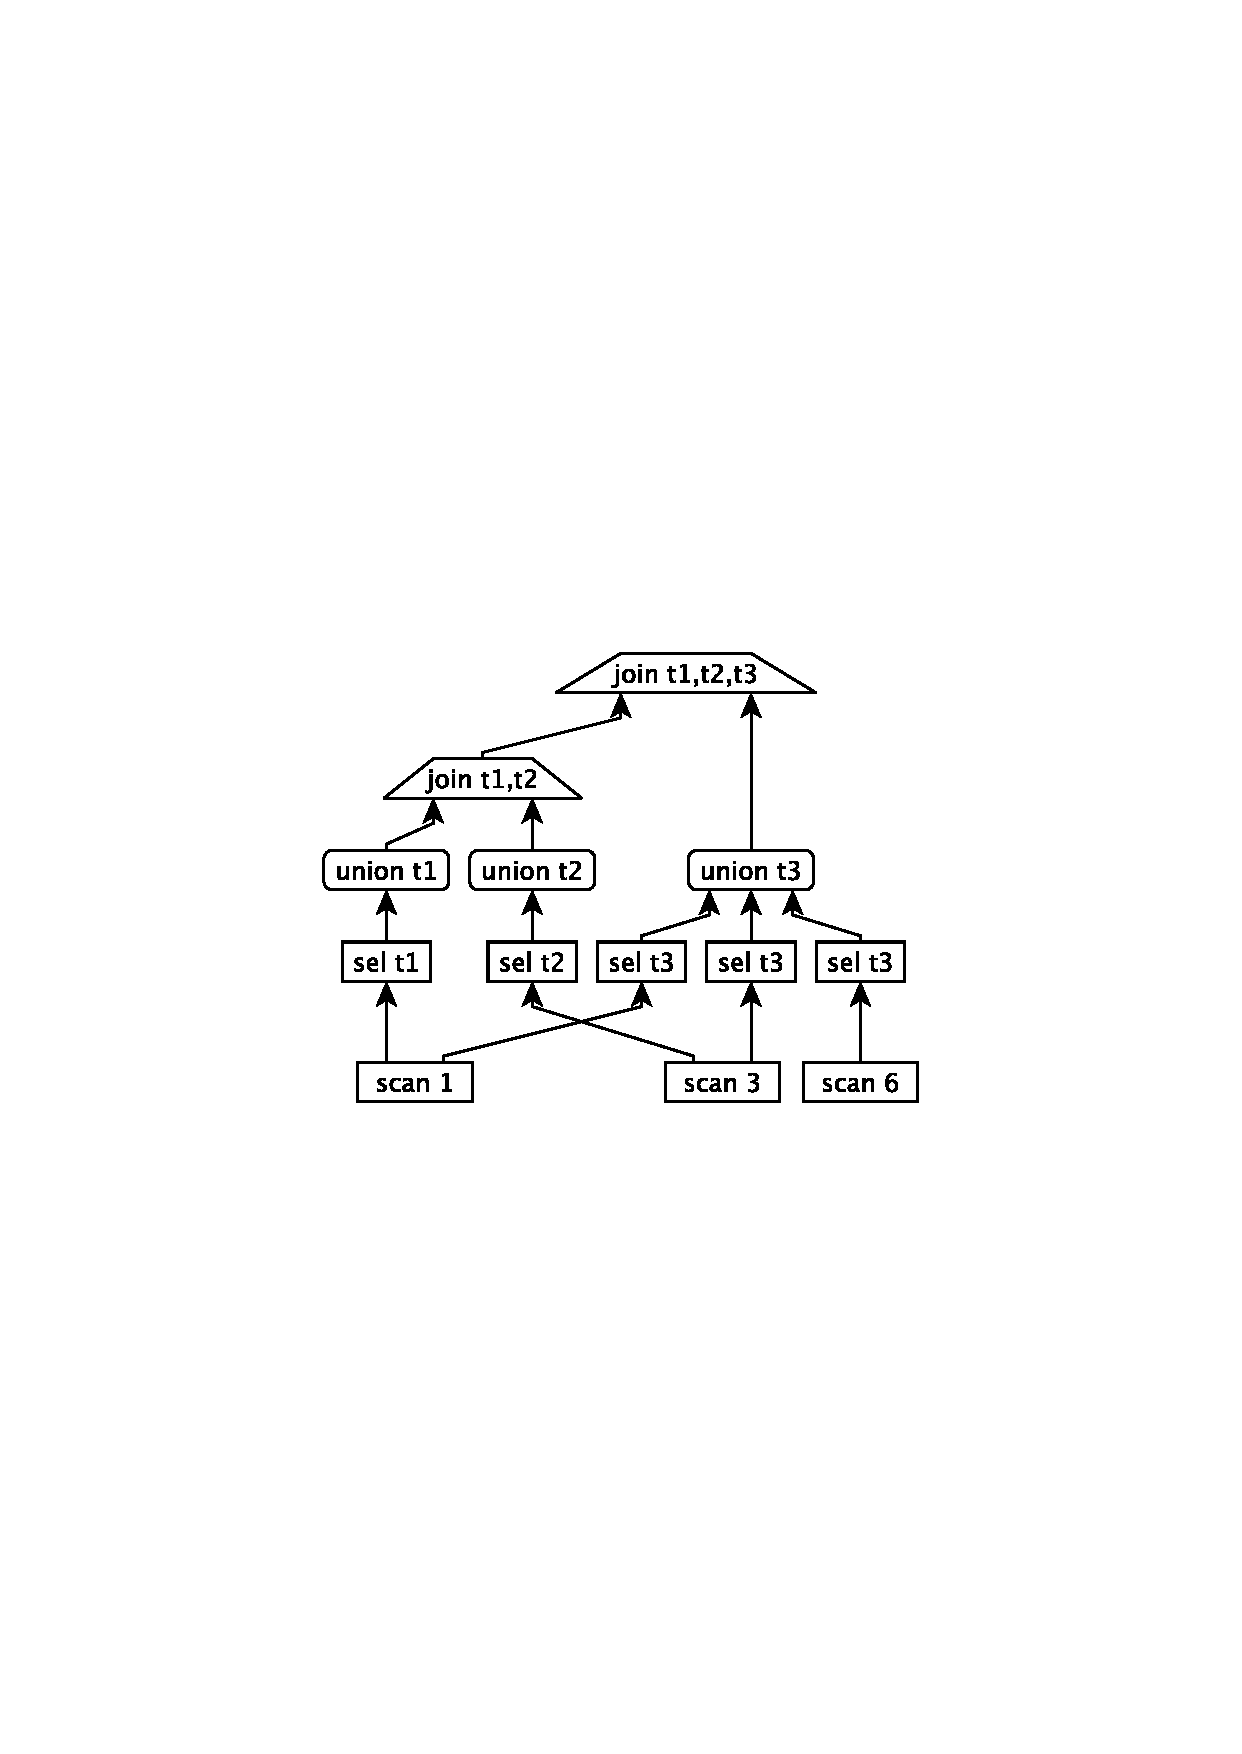
\includegraphics[width=0.6\linewidth]{figs/plan.pdf}
  \caption{Query plan for a query with three triple patterns and two
    sources.}
\label{fig:plan}
\end{figure}

\begin{example}
  Fig.~\ref{fig:plan} shows an example query plan for a query
  consisting of three triple patterns $t_1,t_2,t_3$ and two 
  sources $s_1,s_2$. There are six source scan operators $s_1^{t_1},
  s_2^{t_1}, s_1^{t_2}, \ldots$ for all combinations of triple
  patterns and sources. The source scan operators also have a rank,
  determining their processing order (here $s_2^{t_1}$ is processed
  first). The output of the unions for each triple pattern are joined
  using two symmetric hash joins. \dtr{Fig. not clear}
\end{example}


\subsection{Pareto Optimal Plans} 
Optimality is not clearly defined in the Linked Data context. Traditionally, completeness is assumed such that all results have to be computed. Optimality in this case is defined with respect to processing cost, and optimization techniques aim to find plans that are cost-optimal, i.e. produce all results at lowest costs. As discussed, completeness is not practical in Linked Data query processing and existing approaches (select and) process only a few sources~\cite{harth_data_2010,ladwig_linked_2010}. Not only cost but also the number of results have to be considered here. Further, other criteria such as the trustworthy of sources and the quality of data may play an important role. This results in a \emph{multi-objective} optimization problem. 

For a query $Q$, % = \{t_1, \ldots, t_n\}
the goal is to compute the skyline (Pareto set) of query plans that represent different trade-offs between multiple objectives. For clarity of presentation, we will focus on the two main objectives of maximizing \emph{output cardinality}, $card(\cdot)$, and \emph{processing cost} $cost(\cdot)$. Further, we define cost as $score(\cdot) = \frac{1}{cost(\cdot)}$ such that the objective is to maximize the score and output cardinality.  \todo{use cost instead of score everywhere}
The skyline of a set of solutions is defined using a \emph{dominance}
relation that relates the multiple objectives. A query plan is considered to dominate another plan, if it is at least as good in all objectives and better in at least one objective:

\begin{definition}[Dominance]
  Given two query plans $p_1,p_2$, $p_1 \mbox{ \textnormal{dominates}
  } p_2$ ($p_1 > p_2$) if both, score and cardinality, of $p_1$ are greater or equal
  to the score and cardinalty of $p_2$ and either score or
  cardinality is strictly greater than the score or cardinality of
  $p_2$, i.e. $score(p_1) \geq score(p_2) \wedge card(p_1) \geq
  card(p_2) \wedge ((score(p_1) > score(p_2) \vee card(p_1) >
  card(p_2)) \Rightarrow p_1 > p_2$.
\end{definition}


\begin{definition}[Pareto Optimal Plans]
  Given an query $Q$ and a set of query plans $P(Q)$, the \emph{Pareto}
  set $P^*(Q) \subseteq P(Q)$ comprises all plans that are not
  dominated by any other plan in $P(Q)$, i.e. $P^*(Q) = \{p_i \in P(Q) | \neg\exists p_j\in P(Q), p_j  > p_i\}$. We denote the set of
  dominated plans as $P^-(Q) = P(Q) \setminus P^*(Q)$. The set of \emph{optimal plans} for a query $Q$, denoted as $P^+(Q)$, is the Pareto set of plans for $Q$, i.e. $P^+(Q) = P^*(Q)$.
\end{definition}


\section{Dynamic Programming Based Optimization}
\label{sec:opt}
In this section we propose how to adopt the dynamic
programming (DP) solution~\cite{selinger_access_1979} to the 
multi-objective Linked Data query optimization problem. 

DP for query optimization works in a
bottom-up fashion, constructing the query plan starting from the
leaves, which are scan operators to access
relations. DP is used to deal with the
exponentially large search space of possible query plans. It takes
advantage of the \emph{optimal substructure} of the query optimization
problem, i.e. the optimal query plan can be constructed from
optimal subplans such that non-optimal subplans can be
discarded during the process to reduce the search space.


Applied to Linked Data query processing, we propose to construct access plans $P(t)$ for every triple pattern $t \in Q$. These \emph{atomic plans} are then successively combined 
%using join operators 
to create \emph{composite plans} for larger subexpressions $T \subseteq Q$. 
For instance, to construct a query plan for the expression $T=t_1\Join t_2$, the optimizer may consider all possible pairs $\{(p_1,p_2) | p_1 \in P(t_1),p_2 \in P(t_2)\}$ as possible combinations of plans. When combining two plans $p_1,p_2$ to form a new plan $p$, we
write $p = \mathtt{cmb}(p_1,p_2)$. At each stage, the optimizer 
tries to reduce candidate subplans by discarding those that cannot be part of an optimal solution. That is, before constructing plans for larger subexpressions the optimizer creates $P^+(T) \subseteq
P(T)$, the set of optimal plans for every subexpression $T$. 
%In the case of Linked Data
%query processing, the optimality of a plan is determined according to
%multiple objectives. 

%, i.e., the set of optimal plans is the set of
%Pareto-optimal plans, $P^+(T) = P^*(T)$.

In the following, we firstly discuss how to estimate the optimality of atomic plans as well as composite plans for any expressions $T \subseteq Q$. Then we discuss the main problems that arise when applying the DP solution to this problem of multi-objective Linked Data query optimization.  Because query plans are no longer required to produce all results, we will
discuss a \emph{relaxation of the comparability constraint}. Then, we study the effect of \emph{operator sharing} on query optimization and introduce upper and lower bounds on subplans'
costs. Finally, we prove that the resulting multi-objective query optimization problem still has optimal
substructure and that the proposed dynamic programming solution constructs the
optimal solution, i.e. the skyline of query plans.

\subsection{Estimating Cost and Cardinality of Plans}
\label{sec:estimation}
For the presented structure of a Linked Data query plan and its operators, many existing techniques can be used to systematically estimate cost \cite{stocker_sparql_2008,neumann_scalable_2009,huang_selectivity_2010}. An essential factor for cost estimation is cardinality. While not only input cardinality but also output cardinality are actually used for estimating the cost of some operators, optimizing based on cost alone does not guarantee that the resulting plans are also optimal with respect to output cardinality. 
%Instead of cardinality, the work discussed here is also applicable to other 
%In fact, not 
%%Further, other optimization objectives such as 
%only cost and cardinality but other objectives such as quality and relevance, which may have even smaller overlap with cost, have 
%Thus, estimating the optimality of a plan requires 
%For certain operators, input cardinality is not the same as 

%In this case, not only the cost but also the output cardinality are associated with query operators. 
We will now discuss straightforward estimates that will be needed in this work (and refer the readers to more specific work on cost and join size estimation for more advanced techniques \cite{stocker_sparql_2008,neumann_scalable_2009,huang_selectivity_2010}):

\textbf{Operators.} The output cardinality of the source scan operator is the same as the size of the source, i.e. $card(scan_d) = |T^d|$. 
% If the source is not locally available, it will be
%retrieved remotely. 
%A Linked Data source may contain arbitrary
%data and may therefore contain inputs for other triple
%patterns. If the source scan is an input for more than one operator,
%the data will only be retrieved once and will then either be kept in a
%local buffer for subsequent scans or, in the case of push-based
%execution, immediately be pushed to all subsequent operators.
This source size statistics can be directly obtained from the source index discussed before. 
For union, cardinality is the sum of the cardinalities of its inputs: $card(\cup(I_1,...,I_n)) = \sum_{i=1}^n card(I_i)$. 
The cardinality for selection and join depends on selectivity estimates $sel(\cdot)$, i.e. $card(\sigma_{T^d}(t)) = sel(t) \times |T^d|$ and $card(t_i \Join t_j) =
sel(t_i \Join t_j) \times card(t_i) \times card(t_j)$, respectively. 
%\textbf{Join.} The output cardinality of a join between triples obtained for the two patterns $t_i,t_j$ is given by its selectivity: 
Costs for scan, selection, union and join are $cost(scan_d) = h_s \times |T^d|$, $cost(\sigma_{T^d}(t))=h_\sigma \times |T^d|$, $cost(\cup) =
h_\cup \times card(\cup)$, and $cost(\Join)$ $=
h_\Join \times card(\Join)$, respectively. Thus, cost is assumed to be proportional to cardinality but different weights $h_s,h_\sigma,h_\cup$, and $h_\Join$ are used for different operators. The weight factor $h_\Join$ for instance, depends on the
join algorithm employed. As in previous work on Linked Data query processing, we use symmetric hash join~\cite{ladwig_linked_2010,sihjoin_2011}. In case of operator sharing, separate cost
models for the first source scan (when the data is retrieved over the
network) and subsequent scans (when the data has already been
retrieved) are used. We use $cost_2(scan_d) = (1 - b) \times cost_1(scan_d)$, where $cost_1$ denotes first time cost, $cost_2$ stands for cost for each subsequent scan, and $b$
is a parameter to control the benefit achievable through operator sharing.


\textbf{Atomic Plan.} The cardinality of an access plan $p(t)$ is captured by its root node, i.e. $card(p(t)) = card(\cup_t)$. Its cost is calculated as the sum of the cost of its nodes. Source scan operators are marked after first time usage so that the right cost model can be determined for this calculation. 

\textbf{Composite Plan.} Composite plans capture the joins between results obtained for several triple patterns (outputs of access plans). Thus, for an expression $T = t_i\Join t_j$, $card(p(T))  = card(t_i\Join t_j)$ and $cost(p(T))  = cost(t_i\Join t_j)$.


\subsection{Comparability}
\label{sec:comparability}
% The dynamic programming algorithm works in a bottom-up fashion,
% constructing the query plan starting from the leaves, which in the
% classic problem are scan operators to access relations. Dynamic
% programming is used to deal with the exponentially large search space
% of possible query plans. It takes advantage of the optimal
% substructure of the classic query optimization problem, i.e., the
% optimal query plan can be constructed from optimal sub-plans. This
% enables the optimizer to prune non-optimal plans at each stage and
% only retain optimal sub-plans, reducing the search space
% significantly.

Pruning suboptimal plans is an essential part of the dynamic programming solution to
query optimization. 
%However, the optimizer must take care not to
%discard plans that may be part of an overall optimal solution, which
%then would no longer be found. 
For this, the notion of \emph{comparability} was introduced, which is an equivalence relation $\sim$ over plans. It determines which plans are comparable, based on which  
% according
%to some pre-defined properties. 
the optimizer can decide which plans are suboptimal. The optimizer can prune all but the optimal plans for each of the equivalence classes that are induced by $\sim$. 

In the traditional setting, atomic operators and plans comprising them are \emph{comparable when they produce the same output}. This comparability relation is applicable because input relations are determined by the query such that operators used to process them produce the same output and vary only with regard to cost. The optimizer than chooses how to process data (e.g. table or index
scan) based on cost estimates. In Linked Data query processing, however, the selection of
sources (represented by source scan operators) is part of query
optimization. Thus, the optimizer decides both \emph{what and how data shall be processed}. 
If we apply the comparability concept as defined
previously, each unique combination of source scan operators may yield different results and thus, would be represented by a separate equivalence class of query plans. Given there
are potentially hundreds of Linked Data sources for a single query, this may result in a very large search space. 
% where query optimization is no longer affordable.

However, we note that given the objectives here are cardinality and cost, we are not interested in which results but how many results will be produced. 
%is no longer required, 
Accordingly, a relaxation of this comparability relation can be employed that enables the optimizer to prune plans
more aggressively.

\begin{definition}
  \label{def:comparability}
  Two query plans $p_i, p_j$ are \emph{comparable} if they produce results for the same expression, i.e. $p_i(T_i) \sim  p_j(T_j)$ if $T_i = T_j$. 
\end{definition}

This relaxation means that comparable plans produce the same type of results (bindings for the same pattern), but may vary in the number as well as the actual results produced (different bindings). 

Besides results, other aspects have been incorporated into the comparability relation. For instance, plans may be considered comparable when they produce same results (same type of results), and these results are ordered \dtr{cite}. 
%when considering orders: a non-optimal sub-plan might produce ordered output, which can
%be efficiently used by sort-merge joins later in the query plan and
%should therefore not be discarded at the first possibility.
%Considering other properties such as interesting orders, is of course
%possible, but 
Besides this aspect of interesting orders, the inclusion of other objectives such as relevance and quality would also require a different notion of comparability.  
%For clarity, we omit additional constraints that may be added to. 

\subsection{Monotonicity}
\label{sec:sharing}
% As discussed, the query optimization algorithm based on dynamic
% programming constructs optimal plans for a given query $Q$ by starting
% with plans for single triple patterns $t \in Q$ and successively
% combining plans $P(T_1), P(T_2)$ for subexpressions $T_1,T_2 \subset
% Q, T_1 \cap T_2 = \emptyset$ to create plans $P(T)$ for subexpressions
% $T = T_1 \cup T_2$. In order to minimize the search space when
% creating plans $P(T)$, we prune plans from $P(T_1), P(T_2)$ that
% cannot be part of an optimal plan for $T$.

% In query optimization for relational databases, a plan is usually
% considered to be optimal if it has the lowest cost. Therefore it is
% possible to prune all but one plan for each equivalence class (as
% defined in the previous section) to obtain the set of optimal plans
% $P^*(T)$ for a given expression $T$. For optimization of Linked Data
% queries, however, there are two reasons why this is not as simple: 1)
% we no longer use a single dimension (such as cost) to assess query
% plans, but multiple dimensions (cost and cardinality) and 2) we employ
% operator sharing, which means that the cost function is no longer
% monotonic with regard to combining query plans. We tackle the problem
% of constructing Pareto-optimal query plans in the next section. Here,
% we consider each dimension separately and examine the effect of
% operator sharing on query optimization using dynamic programming.

A central requirement for the DP solution here is that the scoring function must be \emph{monotonic} with respect to plan combination. 
%Without this, the problem no longer has optimal substructure \todo{find something we
%  can cite for this}. 
Only then, subplans can be pruned because it can be guaranteed that they cannot be part of optimal plans. Here, plans have to be compared with respect to different objectives. We will now discuss the monotonicity of the functions employed for cost and cardinality. 
%Given monotonic functions for every 
%This still holds in the context of

\textbf{Cardinality.} Atomic plans are combined to capture joins between results. The monotonicity of the cardinality function can be established because the cardinality function for join is monotonic:

\begin{lemma}
  Given a query $Q$, let $T,T' \subset Q$ be two subexpressions of
  $Q$, such that $T \cap T' = \emptyset$. Let $p_1,p_2 \in P(T)$ and
  $p' \in P(T')$ be plans for $T$ and $T'$. Then we have $card(p_1) \leq
  card(p_2) \Rightarrow card(\mathtt{cmb}(p_1,p')) \leq
  card(\mathtt{cmb}(p_2,p'))$.
\end{lemma}
\begin{proof}
  % The output cardinality of combined plan is determined by the input
  % cardinality (i.e., the output cardinality of the two combined plans)
  % and the selectivity of the join operator used to combined the two
  % plans.
  The plan combinations above capture the expression $T \Join T'$. According to the function $card(T \Join T')$, we can write the condition in
  the theorem as $card(p_1) \leq card(p_2) \Rightarrow card(p_1)
  \times card(p') \times sel(T \Join T') \leq card(p_2) \times card(p') \times
  sel(T \Join T')$. This is true due to monotonicity of multiplication.
\end{proof}

\textbf{Cost.} For cost estimation, operator sharing is taken into
account. Because the costs of first and subsequent scans vary, the
cost of the source scan operator changes when a plan is combined with
another plan that shares that operator.
%Monotonicity is not clear which may cause
%the optimizer to miss the overall optimal plan.
Suppose we have two plans $p,p'$ for the subexpression $T \subset Q$, $cost(p) > cost(p')$,
and a plan $p_t$ for a triple pattern $t$ such that $Q = T \cup
t$. The optimizer would consider $p'$ to
be the optimal plan for $T$ and discard $p$ to form
$P^+(T)=\{p'\}$. Now, because of operator sharing it is possible that
the cost of the combination of two plans is less than the sum of the
cost of the two combined plans, i.e. it is possible that
$cost(\mathtt{cmb}(p,p_t)) < cost(\mathtt{cmb}(p',p_t))$ if $p$ and
$p_t$ share the same source such that the cost of $p_t$ when combined
with $p$ is much lower than the cost of $p_t$ that is combined with
$p'$. In this case, $p'$ is not part of $P^+(T)$.

% To avoid this problem, We need to make sure that the cost and
% cardinality functions are \emph{monotonic} with regard to plan
% combination, meaning that the following conditions must hold:
% \[ cost(p_1) \leq cost(p_2) \Rightarrow cost(\mathtt{cmb}(p_1,p'))
% \leq cost(\mathtt{cmb}(p_2,p')) \]
% \[card(p_1) \leq card(p_2) \Rightarrow card(\mathtt{cmb}(p_1,p'))
% \leq card(\mathtt{cmb}(p_2,p'))\]
% \todo{should we add a proof that the monotonicity of the card function
%   is not violated when employing operator sharing?}

\textbf{Cost Bounds for Partial Plans.} In order to take this effect
of operator sharing into account when calculating the cost of a
partial plan $p$, we define upper and lower bounds for $p$ based on
larger plans that use $p$ as subplans:

\begin{definition}[Lower and Upper Bound Cost]
  \label{def:bounds}
  Given a query $Q$, the subexpressions $T \subset Q$, $T' = Q
  \setminus T$, a plan $p \in P(T)$, and let $P^p(Q) \subseteq P(Q)$
  be the set of all plans for $Q$ that are constructed as combinations
  of $p$ and plans in $P(T')$: $P^p(Q) = \{\mathtt{cmb}(p,p') | p' \in
  P(T')\}$.  Then, we have \emph{lower bound cost} for $p$ as
  $cost_L^Q(p)= MAX\{cost(p)| p \in P^p(Q)\}$ and \emph{upper bound
    cost} for $p$ as $cost_L^Q(p)= MIN\{cost(p)| p \in P^p(Q)\}$.
\end{definition}

Intuitively, a plan $p_i$ for a subexpression $T$ of $Q$ is ``worse''
in terms of cost than another plan $p_j$ for $T$, if all plans for $Q$
that are based on $p_i$ have higher cost than all plans for $Q$ that
are based on $p_j$, i.e., if $cost_L^Q(p_i) > cost_U^Q(p_j)$. Based on
these bounds, we can establish the monotonicity of plan cost with
respect to plan combination as follows:
  
\begin{lemma}
  Let $T,T' \subset Q$ be two subexpressions of $Q$ such that $T \cap
  T' = \emptyset$, and $p_1,p_2 \in P(T)$ and $p' \in P(T')$ be plans
  for $T$ and $T'$, respectively. We have
    \[ cost^Q_U(p_1) \leq cost^Q_L(p_2) \Rightarrow
    cost^Q_U(\mathtt{cmb}(p_1,p')) \leq
    cost^Q_L(\mathtt{cmb}(p_2,p')) \]
\end{lemma}
\begin{proof}
%  This follows directly from the definition of $cost^Q_L$ and
%  $cost^Q_U$ in Def.~\ref{def:bounds}. 
  Any plan for $Q$ that is
  constructed as the combination $p'_1 = \mathtt{cmb}(p_1,p')$, i.e.,
  any plan in $P^{p'_1}(Q)$, is also a $p_1$-combination %  (because
%  $p'_1$ is a combination of $p_1$). From this follows 
such that $P^{p'_1}(Q) \subseteq P^{p_1}(Q)$ and thus, $cost^Q_U(p'_1) \leq
  cost^Q_U(p_1)$. Analogously, for $p_2$ and $p'_2 = \mathtt{cmb}(p_2,p')$, we have $cost^Q_L(p'_2) \geq cost^Q_L(p_2)$. Hence, $cost^Q_U(p_1) \leq cost^Q_L(p_2) \Rightarrow
  cost^Q_U(p'_1) \leq cost^Q_L(p'_2)$. 
%  , meaning the lemma is true.
\end{proof}

Based on these results for cardinality and cost monotonicity, we now
refine the dominance relation to make it applicable to subplans,
i.e. plans for strict subexpressions of $Q$:

\begin{theorem}
  \label{def:dominates_bound}
  Given a query $Q$, a subexpression $T \subset Q$ and two plans
  $p_1,p_2$ for $T$, $p_1 > p_2$ if
  $card(p_1) \geq card(p_2) \wedge cost_U^Q(p_1) \leq cost_L^Q(p_2)
  \wedge (card(p_1) > card(p_2) \vee cost_U^Q(p_1) < cost_L^Q(p_2))$.
\end{theorem}

This is the main result needed for pruning. A subplan is suboptimal
and thus can be pruned if it is dominated in the sense specified
above.

% With the lower and upper bounds we can reestablish the monotonicity of
% plan costs, however in a less restrictive form:

% \begin{theorem}
%   Given two plans $p_1,p_2$ for a subexpression $T$ and a plan $p'$
%   for a subexpression $T'$, such that $T \cap T' = \emptyset$, the
%   following condition holds:
%   \[ cost_U^{T\cup T'}(p_1) \leq cost_L^{T\cup T'}(p_2) \Rightarrow 
%   cost(\mathtt{cmb}(p_1,p') \leq cost(\mathtt{cmb}(p_2,p')) \]
% \end{theorem}
% \begin{proof}
%   \todo{proof}
% \end{proof}

\textbf{Cost Bound Estimation.} 
%In the form of
%Definition~\ref{def:bounds}, 
A basic strategy to compute the lower and upper
bounds of a plan $p$ presented above is to construct all plans based on
$p$. This is of course very cost intensive and defeats the purpose of pruning. Observe that for pruning, we need only to compare the upper and lower bounds between pairs of plans $p_1,p_2$ for the subexpression $T \subset Q$. Given $p_1$, $p_2$ can be pruned if it has higher cost when used to process $T$, and further, when its benefit that may arise when processing other parts of the query cannot outweigh this difference in cost. If exists, this benefit can be completely attributed to operator sharing. Hence, for the efficient estimation of bounds, we propose to focus on the maximal possible benefit that is achievable through operator sharing. As source scan is the only shareable operator, we can derive the maximal benefit by looking at the overlap among all sources that contain data for the query. In particular, only those source scans captured by $p_2$ that are not covered by $p_1$ (i.e. the potential lost when $p_2$ is discarded) have to be considered: 

%As the source scan operator is the only shareable operator, we can
%calculate the maximal possible benefit for a particular plan $p$ by
%using the source index to retrieve all sources for triple patterns not
%covered by $p$ and aggregating the benefit for all sources that are
%also used by $p$.
%
%We only use the maximal benefit when comparing two plans $p,o$ to decide
%whether one plan dominates the other. In this case, we can obtain more
%a more precise benefit $p$ by only aggregating the benefit for sources
%that are not part of $o$. We therefore define the maximal benefit of a
%plan $p \in P(T)$ in terms of another plan $o \in P(T)$:

% \todo{we need to add a proof here that using the bound estimation
%   instead of the real bounds does not prune any plans that shouldn't
%   be pruned. This can be done by saying using the benefits as presented above equals to using bounds. This is the case because the gap between bounds and actual cost express equals benefit, and the only benefit that exists is due to source scan, which is captured above.}
  
  
\begin{definition}[Maximal Benefit]
  Given a query $Q$ and two query plans $p_1,p_2 \in P(T), T \subset Q$, let $D_{p_1},D_{p_2}$ be the sets of sources (i.e. the source scan operators) used by $p_1$ and $p_2$, respectively, $D'_{p_2}$ be the set of sources used by $p_2$ not covered by $p_1$, i.e. $D'_{p_2} = D_{p_2} \setminus D_{p_1}$ and $Q'$ be the set of triple patterns not covered by $p_1$ and $p_2$, i.e. $Q' = Q \setminus T$, the \emph{maximal benefit} of $p_2$ given $p_1$ is $mb(p_2|p_1) = \sum_{t \in Q'}
  \sum_{d \in source(t), d \in D'_{p_2} } b \cdot cost_1(scan_d)$.
%  , where $b$ is the sharing benefit and
%  $cost_1(scan_d)$ is the cost for the first scan
%  of $d$.
\end{definition}

\begin{lemma}
  \label{def:estimated_bound}
  Given a query $Q$, a subexpression $T \subset Q$ and two plans $p_1,p_2$, if $cost(p_1) \leq cost(p_2) - mb(p_2|p_1)$ then $cost_U^Q(p_1) \leq cost_L^Q(p_2)$.
\end{lemma}

%  $p_1,p_2 \in P(T)$, then $p_1 \mbox{\textnormal{ strictly dominates
%    }} p_2$ ($p_1 >_b p_2$) if $card(p_1) \geq card(p_1) \wedge
%  cost(p_1) \leq cost(p_2) - m_{p_1}(p_2) \wedge (card(p_1) >
%  card(p_2) \vee cost(p_1) < cost(p_2) - m_{p_1}(p_2))$.  Whenever
%  $p_1$ strictly dominates $p_2$ then $p_1$ dominates $p_2$: $p_1 >_b
%  p_2 \Rightarrow p_1 > p_2$.
%\end{theorem}
%\begin{proof}
%  We show that if $p_1 >_b p_2$, then $cost^Q_U(p_1) \leq
%  cost^Q_L(p_2)$. If $p_1$ strictly dominates $p_2$ then $cost(p_1)
%  \leq cost(p_2) - m_{p_1}(p_2)$.
%\end{proof}
%>>>>>>> .r564
%
%<<<<<<< .mine
  
Based on these bounds defined with respect to the maximal benefit, we finally obtain the following dominance relation for
pruning subplans:

\begin{theorem}
  Given a query $Q$, a subexpression $T \subset Q$ and two plans
  $p_1,p_2 \in P(T)$, $p_1 > p_2$ if
  $card(p_1) \geq card(p_2) \wedge cost(p_1) \leq cost(p_2) -
  mb(p_2|p_1) \wedge (card(p_1) > card(p_2) \vee cost(p_1) <
  cost(p_2) - mb(p_2|p_1))$.
\end{theorem}


\subsection{Pareto-optimality}
\label{sec:pareto}

The goal of the optimizer in Linked Data query processing 
is to find the overall skyline (or Pareto set) of query plans, while
pruning as many plans as possible at each step. We show that pruning suboptimal plans based on the dominance relation established previously yields the complete Pareto set $P^*(Q)$, i.e., we show that the optimization
problem still has optimal substructure.
%The goal is to find the optimal solution for query $Q$, in this case
%the optimal solution is the set of Pareto-optimal query plans $P^+(Q)
%= P^*(Q)$. 
Given the decomposition of $Q$ into the subproblems $T \subset Q$, we show that we can construct $P^*(Q)$ as a combination of optimal subsolutions $P^*(T)$.  This means a
non-optimal solution for a subproblem $T$ must not be part of an optimal
solution for $Q$:
% The smallest subproblem is a singleton subset of $Q$, i.e., a single
% triple pattern $t$. An optimal solution for this problem is a set of
% Pareto-optimal plans $P^*(\{t\})$. Each such plan $p_t$ is an access
% plan, consisting of a set of source scan operators, whose output is
% fed into separate selection operators and then into a single union
% operator.

% The first step where solutions for subproblems are combined is
% constructing query plans for 2-element subsets of $Q$, i.e., joins
% between base inputs. We show that we can construct $P^*(\{t_1,t_2\})$
% by combining optimal solutions for $t_1$ and $t_2$, i.e.,
% $P^*(\{t_1\})$ and $P^*(\{t_2\})$, for all $t_1,t_2 \in Q$ with $t_1
% \neq t_2$. Let $S$ be the set of all plans constructed by combining
% Pareto-optimal plans for $t_1$ and $t_2$: $S =\{\mathtt{cmb}(p_1,p_2)
% | p_1 \in P^*(t_1), p_2 \in P^*(t_2)\}$. Then we need to show that
% $P^*(\{t_1,t_2\}) = S^*$ or $P^*(\{t_1,t_2\}) \subseteq S$.

% \begin{align*}
%   P^*(\{t_1,t_2\}) \subseteq S &  \Leftrightarrow  \forall p^* \in
%   P^*(\{t_1,t_2\}) : p^* \in S \\
% &   \Leftrightarrow \forall p^* \in P^*(\{t_1,t_2\}) :
%   p^* = \mathtt{cmb}(p^*_1, p^*_2) \;\mathrm{with}\; p^*_1 \in
%   P^*(t_1), p^*_2 \in P^*(t_2)
% \end{align*}

% This means that all optimal, i.e., non-dominated, plans for $t_1,t_2$
% are a combination of non-dominated plans for $t_1$ and $t_2$,
% respectively.

% \todo{benutz kosten ohne bounds hier, oben dann beweisen dass wir beim
%   benutzen der bounds beim prunen irgendwas klappt}

\begin{theorem}
  Given a query $Q$ and two subexpressions $T_1,T_2 \subseteq Q$ with
  $T_1 \cap T_2 = \emptyset$, the set of optimal plans for $T_1 \cup
  T_2$ can be constructed from optimal plans for $T_1,T_2$, i.e.,
  $P^*(T_1 \cup T_2) =
  \{\mathtt{cmb}(p_1,p_2) | p_1 \in P^*(T_1), p_2 \in P^*(T_2)\}$.
\end{theorem}
\begin{proof}
  We prove this by contradiction: Let $p^* \in P^*(T_1 \cup T_2)$ be a plan that is a combination of a
  dominated plan for $T_1$ and a non-dominated plan for $T_2$, i.e.,
  $p^* = \mathtt{cmb}(p^-_1,p^*_2),p^-_1 \in P^-(T_1),p^*_2 \in
  P^*(T_2)$. This means, there must be a non-dominated plan $p^*_1 \in
  P^*(T_1)$ that dominates $p^-_1$, but the combination of $p^*_1$
  with $p^*_2$ is dominated by the combination of $p^-_1$ and $p^*_2$:
  \[ \exists p^*_1 \in P^*(T_1) : \mathtt{cmb}(p^-_1,p^*_2) \text{
    dominates } \mathtt{cmb}(p^*_1,p^*_2)\] Given $p^*_1$ dominates
  $p^-_1$ and $\mathtt{cmb}(p^-_1,p^*_2)$ dominates
  $\mathtt{cmb}(p^*_1,p^*_2)$, it follows from the established dominance relation that
  (without loss of generality, we use strictly lesser/greater relations):
  \begin{eqnarray*}
    card(p^-_1) < card(p^*_1) &\wedge& card (\mathtt{cmb}(p^-_1,p^*_2)) > card(\mathtt{cmb}(p^*_1,p^*_2)) \\
    cost^Q_L(p^-_1) > cost^Q_U(p^*_1) &\wedge& cost^Q_U(\mathtt{cmb}(p^-_1,p^*_2)) < cost^Q_L(\mathtt{cmb}(p^*_1,p^*_2))\\
  \end{eqnarray*}
  However, this contradicts with the monotonicity property established for cost, because $cost^Q_L(p^-_1) >
  cost^Q_U(p^+_1)$, but $cost^Q_U(\mathtt{cmb}(p^-_1,p^*_2)) <
  cost^Q_L(\mathtt{cmb}(p^*_1,p^*_2))$. Analogously, a contradiction also follows from the monotonicity of cardinality. With regard to our original proposition, this means
  that there is no plan $p^* \in P^*(T_1 \cup T_2)$, such that $p^*$
  is a combination of a dominated plan $p^-_1$ and a non-dominated plan
  $p^*_2$. This obviously also holds true when $p^*$ is a combination of two dominated
  plans. Thus, all
  $p^* \in P^*(T_1 \cup T_2)$ must be combinations of non-dominated
  plans in $P^*(T_1)$ and $P^*(T_2)$ and therefore $P^*(T_1 \cup T_2)$.
\end{proof}

% Proof by contradiction: Suppose there is a non-dominated plan $p^* \in
% P^*(\{t_1,t_2\})$ that is a combination of a dominated plan for $t_1$ and
% a non-dominated plan for $p_2$:
% \[\exists p^* \in P^*(\{t_1,t_2\}) : p^* = \mathtt{cmb}(p^-_1,p^*_2),
% p^-_1 \in P^-(t_1), p^*_2 \in P^*(t_2) \] 

% This would mean that there is a non-dominated plan $p^*_1 \in
% P^*(t_1)$ that naturally dominates $p^-_1$, but the combination of
% $p^*_1$ with $p^*_2$ is dominated by the combination of $p^-_1$ and
% $p^*_2$:
% \[ \exists p^*_1 \in P^*(t_1) : \mathtt{cmb}(p^-_1,p^*_2)
% \text{ dominates } \mathtt{cmb}(p^*_1,p^*_2)\]

% This implies that the score and cardinality of
% $\mathtt{cmb}(p^-_1,p^*_2)$ are greater or equal than the score and
% cardinality of $\mathtt{cmb}(p^*_1,p^*_2)$, whereas the score and
% cardinality of $p^-_1$ is less than the score and cardinality of
% $p^*_1$ (because $p^*_1$ dominates $p^-_1$):

% \begin{eqnarray*}
%   score(p^-_1) < score(p^*_1) &\wedge& score(\mathtt{cmb}(p^-_1,p^*_2)) \geq score(\mathtt{cmb}(p^*_1,p^*_2))\\
%   card(p^-_1) < card(p^*_1) &\wedge& card (\mathtt{cmb}(p^-_1,p^*_2)) \geq card(\mathtt{cmb}(p^*_1,p^*_2)) \\
% \end{eqnarray*}

% However, we postulate that $card$ and $score$ are monotonic with
% regard to the combination of plans:
% \begin{eqnarray*}
%   score(p_1) \leq score(p'_1) &\Rightarrow& score(\mathtt{cmb}(p_1,p_2))
%   \leq score(\mathtt{cmb}(p'_1,p_2)) \\
%   card(p_1) \leq card(p'_1) &\Rightarrow& card(\mathtt{cmb}(p_1,p_2))
%   \leq card(\mathtt{cmb}(p'_1,p_2)) \\
% \end{eqnarray*}

% where $p_1,p'_1$ are any plans for the same expression and $p_2$ is a
% plan for a different, disjunct expression. 

% \todo{add bounds here}

% With the monotonicity of the $score$ and $card$ functions we have a
% contradiction, because $score(p^-_1) < score(p^*_1)$, but
% $score(\mathtt{cmb}(p^-_1,p^*_2)) \geq
% score(\mathtt{cmb}(p^*_1,p^*_2))$ (the same holds for the
% cardinality). With regard to our original proposition, this means that
% there is no plan $p^* \in P^*_{t_1,t_2}$ such that $p^*$ is a
% combination of a dominated plan $p^-_1$ and a non-dominated plan
% $p^*_2$. \todo{show that this also holds when both plans are
%   dominated} From this follows that all $p^* \in P^*_{t_1,t_2}$ are
% combinations of the non-dominated plans in $P^*_{t1}$ and $P^*_{t_2}$.


%Although the relaxed comparability constraint allows the optimizer to
%prune more aggressively than otherwise possible, we observe that the
%goal of generating Pareto-optimal query plans again leads to a larger
%search space.

\subsection{Optimizer Algorithm}

In this section we present a DP algorithm that exploits the previously established theoretical results to perform Linked Data multi-objective query optimization. It builds upon the classic DP algorithm. It takes the proposed structure of Linked Data query plans into account, and at each step, uses Pareto-optimality to prune
plans according to the optimization objectives.

% \subsubsection{Pareto-optimal Access Plans for Triple Patterns}

% The first step in the dynamic programming algorithm for query
% optimization is creating Pareto-optimal access plans for single query
% triple patterns. As described in Section~\ref{sec:basicshape} these
% plans each consist of a set source scan operators whose output feeds
% into selection operators and then in a single union operator. Given a
% triple pattern $t$, we first use the source index to obtain the set of
% relevant sources $D = I(t)$.

% A naive solution to obtain the Pareto-optimal plans for $t$ would be
% to first create the set of all possible plans and then prune all
% dominated plans. However, we can construct a valid plan for $t$ from
% any subset of $D$, i.e., there is one possible plan for each element
% of the power set of $D$. As the size of the power set is $2^{|D|}$
% this is infeasible even for triple patterns that appear in only
% relatively few sources.

% \todo{add short description of the algorithm we use}

% \subsubsection{Pareto-optimal Dynamic Programming}

\begin{algorithm}
  \label{alg:plan}
  \DontPrintSemicolon

  \caption{\textsc{PlanGen}$(Q)$}
  \KwIn{Query $Q = \{t_1,\ldots,t_n\}$}
  \KwOut{Pareto-optimal query plans $P^*(Q)$}

  \ForEach{$t \in Q$}{
    $S \leftarrow \{ \cup(\{ \sigma_{T^d}(t) | d \in D \}) | D \in
    \mathcal{P}(source(t))\}$ \;
    $P^*(t) \leftarrow \{p \in S| \nexists p' \in S : p' > p \}$
    \; 
  }

  \For{$i \leftarrow 2$ \KwTo $|Q|$}{
    \ForEach{$T \subseteq Q$ such that $|T| = i$}{
      \ForEach{$t \in T$}{
        $S \leftarrow S \cup \{\mathtt{cmb}(p_1,p_2) | p_1 \in
        P^*(t), p_2 \in P^*(T \setminus t)\}$ \;
      }
      $P^*(T) \leftarrow \{p \in S | \nexists p' \in S : p'
      > p \}$\;
    }
  }
  \Return $P^*(Q)$
\end{algorithm}

Algorithm~\ref{alg:plan} shows the method \textsc{PlanGen} that takes
a query $Q=\{t_1,\ldots,t_n\}$ as input and
returns the Pareto-optimal plans for $Q$. During optimization, $P^*$
stores the optimal plans for subexpressions of $Q$.

In the first step, access plans for single triple patterns are created
(lines 1-3). For each triple pattern $t$ in $Q$, relevant
sources are determined using the source index. As we need to
consider all possible combinations of sources, we create the power set
$\mathcal{P}(source(t))$ of all sources (line 2). For each member $D$ of
the power set, we create an access plan, consisting of a scan and a selection operator $\sigma_{T^d}(t)$ for each source $d \in D$ and a
single union operator $\cup$ that has the selection operators as
input. $S$ then contains a set of access plans, one for each
combination of relevant sources. From this set, we then select only
the non-dominated, i.e., Pareto-optimal, access plans and store them
in $P^*(t)$ (line 3).

During the next iterations (line 4-8), previously
created plans are combined until all query triple patterns are
covered. For iteration $i$, we select all subsets $T \subseteq Q$ with
$|T|=i$. For each $t \in T$ the algorithm creates all possible combinations
between the best, i.e., Pareto-optimal, plans for $t$ and $T\setminus
t$ (line 7). By selecting only a single triple pattern from $T$ we
create only left-deep plans. Instead, bushy plans may be used.
All these plans are stored in $S$ and are comparable since they cover
the same triple patterns $T$. Finally, only the non-dominated plans
from $S$ are selected and stored in $P^*(T)$ (line 8). After the last
iteration, $P^*(Q)$ contains all the Pareto-optimal plans for
$Q$ (line 9).

\textbf{Complexity.} The join order optimization problem has been
shown to be NP-complete \cite{vance_rapid_1996} and the classic
dynamic programming algorithm for query optimization has a time
complexity of $O(3^n)$ \cite{kossmann_iterative_2000}, where $n$ is
the number of relations (triple patterns in the case of Linked Data
queries) to be joined. Our approach for multi-objective query
optimization adds the dimension of source selection to the query
optimization problem. Given a set of $m$ sources, we can think of the
problem as, in worst case, creating a query plan for each unique
combination of sources, of which there are $2^m$, leading to a
complexity of $O(2^m \cdot 3^n)$. This theoretical worst case complexity does not change in the multi-objective case. However in practice, the number of plans (and combination of sources) that can be pruned at every iteration can be expected to be much larger in the single-objective case, compared to the multi-objective case. Particularly the use of operator sharing leads to a larger amount non-dominated plans. One strategy to deal with that is to approximate the bounds that we have established. In the experiment, we study one basic approximation, which instead of the cost bounds, use actual cost for pruning. That is, it ignores the bounds and accepts the discussed cases where subplans, which become non-optimal through operator sharing, may be part of the final result. 

%\subsection{Discussion: Multi-Objective and Top-K}
% \subsection{Adaptivity}
% The goal of adaptive query processing is to perform query optimization
% in the case were no complete knowledge is available and adapt the
% query processing at run-time by using newly available
% knowledge. During processing of Linked Data queries, new information
% about sources becomes available: 1) new sources may be discovered, 2)
% state accumulated inside join operators can be used to perform better
% estimates of join cardinalities for a particular source and 3) data
% properties may be observer to deviate from previous estimates.

% Here, we adopt techniques from previous research on adaptive query
% processing.

% \todo{what do we monitor? when is re-optimization done?}

% Linked Data query processing requires ranking to be performed not only
% at compile-time, but also continously at run-time in order to take
% advantage of knowledge gained during query processing. Using
% adaptive query processing techniques not only ranking can be
% performed, but full query optimization at run-time. 

% Weight distribution between cost and relevancy might change over time:
% at first, relevancy is more important, while later on, after results
% have been produced, cost becomes more important?


% \subsection{Implementation}
% \label{sec:impl}

% \todo{describe concrete implementation, in particular methods used for
% cost/result estimation and query strategies different from the optimal
% ones}

% \todo{dependencies between sources are not reflected by available
%   statistics, but indirectly captured using run-time reestimation of
%   result sizes using sampling etc.}



%%% Local Variables: 
%%% mode: latex
%%% TeX-master: "paper"
%%% End: 

%\input{section-processing}
\section{Related Work}
\label{sec:related}

\textbf{Linked Data Query Processing.} The concept of executing SPARQL
queries directly over Linked Data instead of a locally indexed copy
was first introduced in \cite{hartig_executing_2009}, where link
traversal is used to discover sources at runtime. In
\cite{harth_data_2010} a local source index based on QTrees is used to
speed up the discovery of relevant sources. Our previous work
\cite{ladwig_linked_2010,sihjoin_2011} proposes methods for
ranking sources at runtime according to their relevancy and a mixed
execution strategy that combines both, link traversal and source
indexes, to report results early. In this work we adopt the approach
from \cite{harth_data_2010} and employ a source index without any
runtime source discovery along with the push-based Symmetric Hash Join
operator from \cite{ladwig_linked_2010,sihjoin_2011}.


% \textbf{Dynamic Programming.}

% Faster enumeration of plans: \cite{moerkotte_analysis_2006,moerkotte_dynamic_2008}

% Iterative Dynamic Programming (approx): \cite{kossmann_iterative_2000}

\textbf{Multiobjective Query Optimization.} Multi-objective query
optimization was previously proposed in
\cite{papadimitriou_multiobjective_2001}, where it is discussed in the
context of Mariposa, a wide-area database system. The Mariposa
optimizer splits the query tree into subqueries and then obtains
\emph{bids} from participating database sites that specify a delay and
cost for delivering the result of a subquery. The goal of the optimzer
is to obtain the Pareto optimal set of plans with respect to cost and
delay. While the authors do employ dynamic programming to show that
the Pareto set can be approximated in polynomial time, it is not based
on the classic dynamic programming algorithm for query optimization
proposed in \cite{selinger_access_1979}. The problem is slightly
different as there is only a single query operation tree and for each
operation node the optimizer is provided a list of alternatives for
implementing the operation. In contrast, the classic dynamic
programming \cite{selinger_access_1979} does not consider only a
single query tree (and therefore a single order of operations), but
builds and optimizes physical query plans from the bottom up and
considers all valid query trees. In this work we extend the classic
algorithm to support multi-objective query optimization.


The approach presented in \cite{nie_joint_2001} optimizes query plans
not only for cost, but also for coverage (i.e. output cardinality) and
thereby integrates source selection into the query optimization
process. However, the optimization is performed by combining
(weighted) cost and coverage into a utility function that provides a
single measure to assess query plans. Using a single measure means
that traditional query optimization algorithms, such as dynamic
programming \cite{selinger_access_1979}, are directly
applicable. However, no true multi-objective optimization is
performed.


\textbf{Data Integration.}

Bucket algorithm: \cite{levy_querying_1996}

MiniCon algorithm: \cite{pottinger_minicon:_2001}

Optimization of cost and coverage (utility function):
\cite{nie_joint_2001}

Source selection: \cite{pomares_source_2010}

Query Planning in the Presence of Overlapping Sources:
\cite{bleiholder_query_2006}

survey materialized views: \cite{halevy_answering_2001}



%%% Local Variables: 
%%% mode: latex
%%% TeX-master: "paper"
%%% End: 

\section{Evaluation}
\label{sec:eva}

The evaluation of our approach consists of two parts. In the first, we
evalute the benefit of using the dynamic programming query
optimization algorithm for Linked Data query processing in a
single-objective scenario. In the second part, we focus on the
multi-objective optimization approach proposed in this paper.

\subsection{Single-objective Optimization with Dynamic Programming}

\subsubsection{Systems}


\subsubsection{Results}



\begin{figure}[htb]
  \centering
  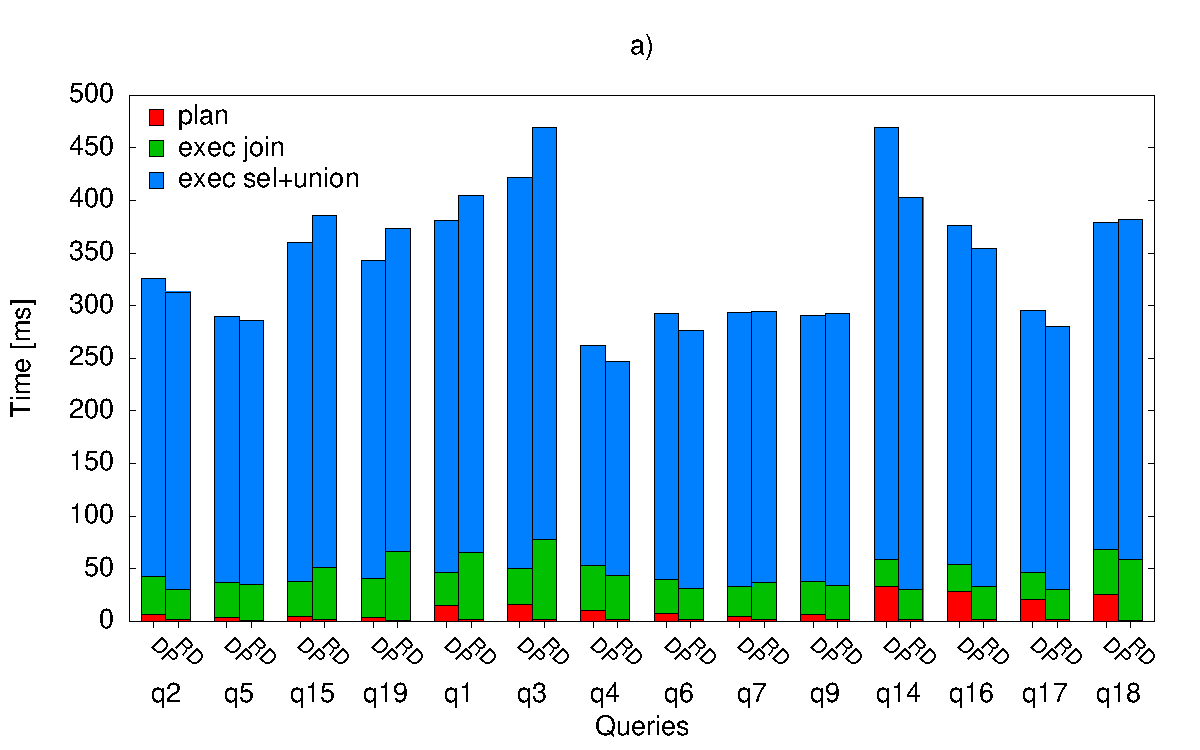
\includegraphics[width=\linewidth]{figs/exec_queries.pdf}
  \caption{Results for execution}
  \label{fig:exec_queries}
\end{figure}


\subsection{Multi-objective Optimization with Dynamic Programming}

\subsubsection{Systems}

\textbf{Baselines.} As there are no comparable source selection and
query optimization approaches that produce a range of query plans
instead of a single one, we implemented two straightforward baselines
in order to evaluate the quality of the plans produced by our new
approach. 

The first baseline (RD) is based on randomly selecting subsets of $D$
with sizes $\{1\ldots |D|\}$ (i.e., there are $|D|$ such subsets). For
each of these subsets, we create a single query plan using a standard
dynamic programming optimizer. Source scan operators are shared
between triple patterns where appropriate.

The second baseline (RK) is simliar to the first one, except that the
sources in $D$ are first ranked by the number of contained triples
that match query triple patterns (as obtained from the source index),
calculated as $score(d) = \sum_{t \in q} card_t(d)$. Instead of a
random selection, we now create subsets of $D$ by starting with the
highest ranked source and then successively adding sources in order of
their ranking to obtain $|D|$ subsets in total. For each subset, we
build a query plan in the same manner as for baseline RD.

\todo{explain modifications to create more plans}

\textbf{Our Approach.} We implemented two versions of our
approach. The first version (DP) obtains the complete set of
Pareto-optimal plans as described in the previous sections. The second
version (DPU) does not use bounds as described in
Section~\ref{sec:sharing} (i.e., while operator sharing is employed,
its effect are not taken into account during pruning) and therefore
will not compute the correct Pareto-optimal set of plans. However,
pruning is more effective and should lead to faster performance.

\textbf{Parameters.} Parameter $b$ specifies the benefit that is
assumed during query planning for sharing of source scan
operators. For example, with $b=0.8$ the planners assume that 80\% of
the source scan cost is saved, i.e., second and subsequent reads of a
source scan operator cost only 20\% of the first read.

For RD and RK, parameter $m$ describes the number of additional plans
that were generated by randomly removing source scan operators.

\subsubsection{Datasets and Queries}

We created 14 BGP queries of different sizes w.r.t. to the number of
triple patterns. We executed all queries using a link traversal
approach and recorded all retrieved sources. This dataset was then
indexed in a source index and used for the evaluation. The dataset
consists of 1,909,109 triples and contains data from various popular
open datasets, such as DBpedia, Freebase, New York Times, GeoNames,
LinkedMDB and others. 

\todo{describe how sources were aggregated to host-sources}

Table~\ref{tab:queries} shows various statistics for all evaluation
queries.

\begin{table}[htb]
  \centering
  \begin{tabular}{l|c|c|r|r|r|r}
    Query & \#Pat. & \#Src. & \#Src./Pat. (SD) & Shared [kT] & \#Res. & Join-Sel. SD \\ 
    \hline

    Q2  & 3 & 13 & 5.33 (6.66) & 1,175 & 24  & 2.36\textsc{e}-5 \\
    Q5  & 3 & 13 & 5.00 (6.93) & 633   & 13  & 5.73\textsc{e}-5 \\
    Q15 & 3 & 13 & 5.33 (6.66) & 1,245 & 11  & 3.95\textsc{e}-5 \\
    Q19 & 3 & 13 & 7.33 (6.03) & 1,329 & 918 & 4.36\textsc{e}-5 \\
    \hline
    Q1  & 4 & 13 & 4.75 (5.56) & 1,296 & 2   & 1.30\textsc{e}-3 \\
    Q3  & 4 & 13 & 4.75 (5.56) & 1,762 & 3   & 1.89\textsc{e}-5 \\
    Q4  & 4 & 13 & 4.00 (6.00) & 50    & 60  & 9.58\textsc{e}-3 \\
    Q6  & 4 & 13 & 4.00 (6.00) & 594   & 6   & 2.62\textsc{e}-3 \\
    Q7  & 4 & 13 & 4.75 (5.68) & 702   & 106 & 2.75\textsc{e}-3 \\
    \hline
    Q9  & 5 & 13 & 4.60 (5.37) & 703   & 17  & 5.26\textsc{e}-3 \\
    Q14 & 5 & 8  & 2.60 (3.05) & 1729  & 20  & 3.71\textsc{e}-3 \\
    Q16 & 5 & 13 & 3.80 (5.22) & 951   & 1   & 2.10\textsc{e}-3 \\
    Q17 & 5 & 13 & 3.40 (5.37) & 599   & 1   & 8.92\textsc{e}-3 \\
    Q18 & 5 & 10 & 3.00 (3.39) & 970   & 2   & 1.21\textsc{e}-4 \\
  \end{tabular}
  \caption{Query statistics: query name, number of patterns, number of unique sources, average number of sources per pattern (standard deviation), number of triples (in thousands) contained in shared sources, number results, standard deviation of selectivies of all joins in query.}
  \label{tab:queries}
\end{table}

\begin{table}[htb]
  \centering
  \begin{tabular}{l|r|r|r|r|r|r|r|r|r|r|r|r|r|r|r|r}
 & RD & RK & DP & DPU & RD & RK & DP & DPU & RD & RK & DP & DPU & RD & RK & DP & DPU \\
    \hline               
                                                                                                               
 & \multicolumn{4}{c}{Q2} & \multicolumn{4}{|c|}{Q5} & \multicolumn{4}{c}{Q15} & \multicolumn{4}{|c}{Q19}  \\

    \hline                                                                                                   

    \#Plans   & 1702 & 1853 & 673   & 619  & 1382 & 1871 & 446   & 446   & 2376 & 3263 & 634   & 634   & 3817 & 3240 & 761   & 761   \\
    \#Skyline & 153  & 155  & 673   & 575  & 106  & 176  & 446   & 446   & 13   & 40   & 634   & 634   & 41   & 46   & 761   & 761   \\ 
    \%Skyline & 22.7 & 23.0 & 100.0 & 85.4 & 23.8 & 39.5 & 100.0 & 100.0 & 2.1  & 6.3  & 100.0 & 100.0 & 5.4  & 6.0  & 100.0 & 100.0 \\
    Time [s]  & 1.06 & 0.92 & 1.14  & 0.62 & 0.78 & 1.03 & 0.75  & 0.53  & 1.05 & 1.14 & 1.21  & 0.64  & 1.07 & 1.05 & 1.58  & 0.77  \\
  
    \hline
    \hline

 & \multicolumn{4}{c}{Q1} & \multicolumn{4}{|c|}{Q3} & \multicolumn{4}{c|}{Q4} & \multicolumn{4}{c}{Q6} \\

    \hline

    \#Plans   & 3945 & 5362 & 866   & 832  & 4571 & 5153 & 901   & 847  & 1471 & 1306 & 453   & 465  & 954  & 1340 & 354   & 318  \\
    \#Skyline & 0    & 0    & 866   & 689  & 0    & 0    & 901   & 699  & 1    & 0    & 453   & 434  & 0    & 1    & 354   & 283  \\ 
    \%Skyline & 0.0  & 0.0  & 100.0 & 79.6 & 0.0  & 0.0  & 100.0 & 77.6 & 0.2  & 0.0  & 100.0 & 95.8 & 0.0  & 0.2  & 100.0 & 79.9 \\
    Time [s]  & 1.53 & 1.67 & 7.64  & 1.60 & 1.53 & 1.62 & 10.05 & 1.80 & 1.61 & 1.29 & 1.37  & 0.75 & 1.14 & 1.33 & 1.35  & 0.70 \\

    \hline
    \hline

 & \multicolumn{4}{c}{Q7} & \multicolumn{4}{|c|}{Q9} & \multicolumn{4}{c|}{Q14} & \multicolumn{4}{c}{Q16} \\

    \hline

    \#Plans   & 2566 & 3913 & 1035  & 813  & 2622 & 3450 & 689   & 655  & 429  & 436  & 284   & 281  & 1485 & 2265 & 685   & 663  \\
    \#Skyline & 1    & 0    & 1035  & 781  & 0    & 0    & 689   & 637  & 0    & 0    & 284   & 281  & 0    & 0    & 685   & 583  \\ 
    \%Skyline & 0.1  & 0.0  & 100.0 & 75.5 & 0.0  & 0.0  & 100.0 & 92.5 & 0.0  & 0.0  & 100.0 & 98.9 & 0.0  & 0.0  & 100.0 & 85.1 \\
    Time [s]  & 1.91 & 1.50 & 20.88 & 2.28 & 1.80 & 1.64 & 23.64 & 2.56 & 1.33 & 1.21 & 0.91  & 0.41 & 1.82 & 1.99 & 14.31 & 2.38 \\

    \hline
    \hline

 & \multicolumn{4}{c}{Q17} & \multicolumn{4}{|c|}{Q18} & \multicolumn{8}{c}{} \\

    \hline

    \#Plans   & 837  & 1022 & 398   & 286   & 1021 & 1192 & 633   & 633   & \multicolumn{8}{c}{} \\
    \#Skyline & 1    & 0    & 398   & 286   & 0    & 0    & 633   & 633   & \multicolumn{8}{c}{} \\ 
    \%Skyline & 0.2  & 0.0  & 100.0 & 100.0 & 0.0  & 0.0  & 100.0 & 100.0 & \multicolumn{8}{c}{} \\
    Time [ms] & 1.67 & 1.70 & 2.68  & 0.66  & 1.53 & 1.58 & 4.15  & 1.35  & \multicolumn{8}{c}{} \\

  \end{tabular}
  \caption{Results for all queries, with $m=2000$ and $b=0.8$ for RD and RK.}
  \label{tab:res}
\end{table}

\subsubsection{Results}

Table~\ref{tab:res} shows an overview of all queries for all systems
with $b=0.8$ and $m=2000$. \todo{add averages here}

\textbf{Effect of Query Size.} Figs.~\ref{fig:pareto_tp}a+b show the
planning time and found skyline fraction for different query sizes
(i.e., number of triple patterns). An increased number of triple
patterns results in a larger search space for the query optimizer: for
all systems planning time increases with the number of triple
patterns. However, the DP algorithm is much more affected than DPU, RK
and RD. Going from 3 to 5 triple patterns, the planning time of DP
increases by a factor of 7.6, whereas the other systems' planning
times only increase by factors between 1.6 (RK) and 2.3 (DPU). 

Fig.~\ref{fig:pareto_tp}b shows the fractions of the complete plan
skyline (i.e., the plans computed by DP) that the systems are able to
calculate for different query sizes. 

\begin{figure}[htb]
  \centering
  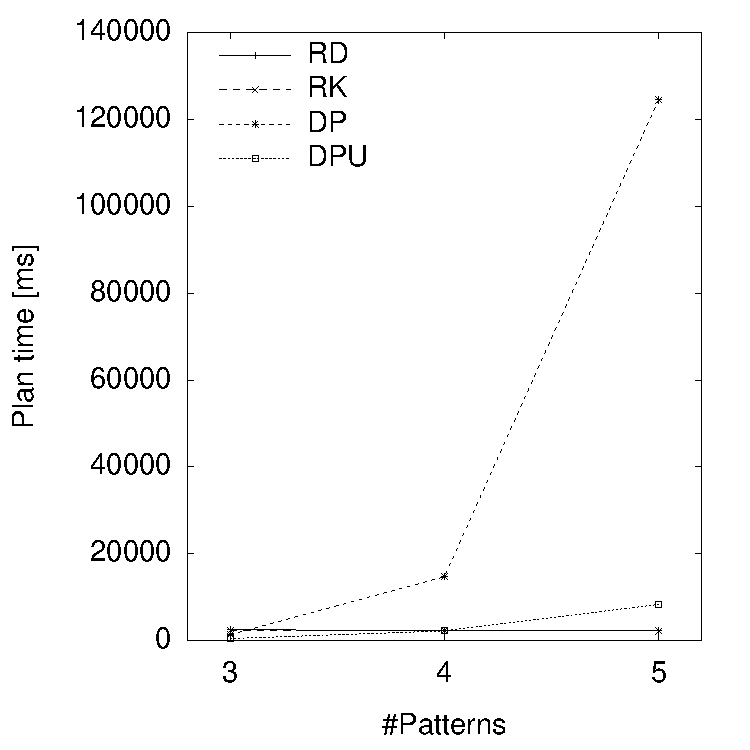
\includegraphics[width=0.49\linewidth]{figs/pareto_plan_tp.pdf}
  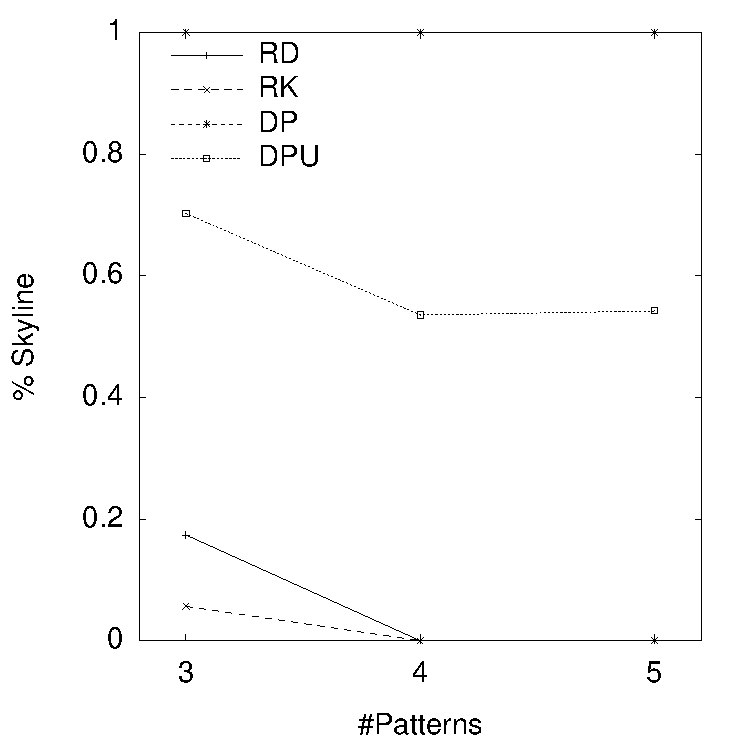
\includegraphics[width=0.49\linewidth]{figs/plans_skyline_by_tp.pdf}
  \caption{Effect of query size on a) planning time and b) skyline fractions.}
  \label{fig:pareto_tp}
\end{figure}

\textbf{Effect of Sharing Benefit.} Figs.~\ref{fig:pareto_sharing}a+b
show the planning time and skyline fractions for different values of
$b$. We see in Fig.~\ref{fig:pareto_sharing}a that the planning time
for DP increases with higher sharing benefits: from 3.3s for $b=0.1$
to 6.4s for $b=0.8$. However, the planning time for the other
approaches, DPU, RD, and RK, remain the same for all values of
$b$. The planning time for DP increases with higher sharing benefits
because the bounds of plan costs are less tight and less plans can be
pruned during the query optimization process. The other approaches are
not affected because DP is the only one that actually considers the
sharing benefit during optimization.

Fig.~\ref{fig:pareto_sharing}b shows the skyline fractions for all
approaches for different values of $b$. We can see that DPU computes a
larger part of the skyline when the sharing benefit is lower. This is
due to the fact that DPU does not take the effect of operating sharing
into account, leading to worse results the more pronounved the
influence of the sharing benefit is. The other approaches, RD and RK,
are not affected by the sharing benefit as the benefit is not taken
into account during planning.

\begin{figure}[htb]
  \centering
  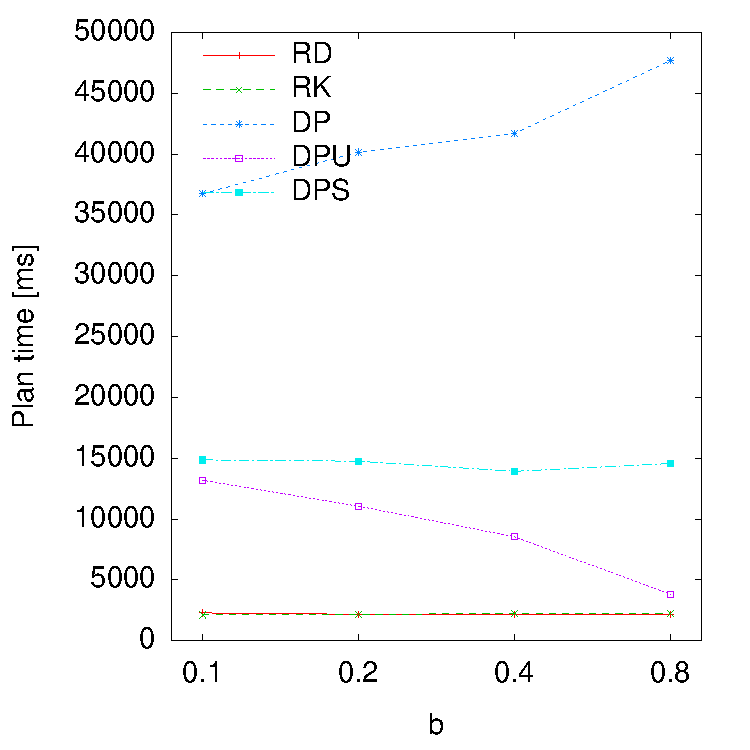
\includegraphics[width=0.49\linewidth]{figs/pareto_plan_b.pdf}
  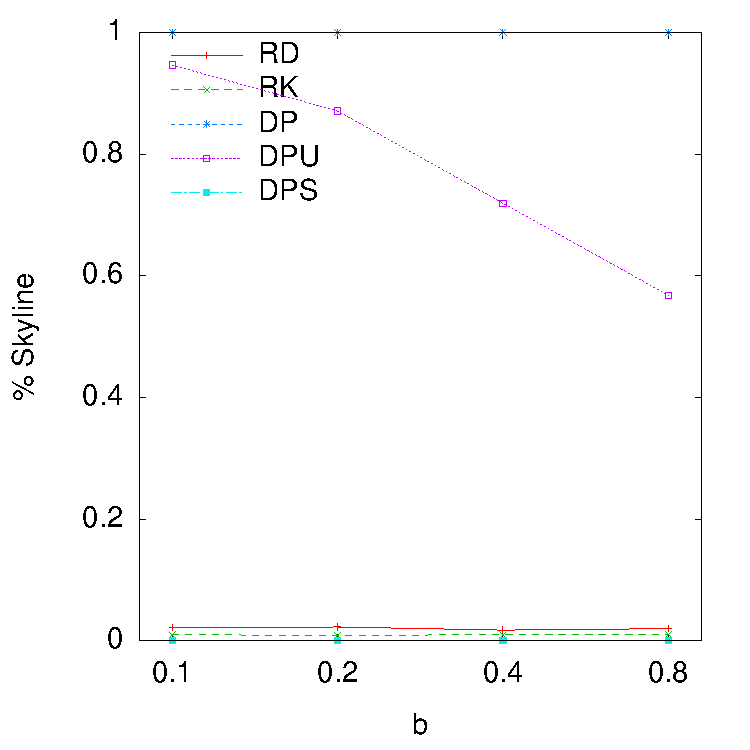
\includegraphics[width=0.49\linewidth]{figs/plans_skyline_by_b.pdf}
  \caption{Effect of sharing benefit on a) planning time and b)
    skyline fractions.}
  \label{fig:pareto_sharing}
\end{figure}

\textbf{Plan Skyline.} Figs.~\ref{fig:pareto_q2_skyline}a+b show a scatter
plot of cost and cardinality of plans generated by all systems for
query Q2. In these plots a plan dominates all plans that are to its
lower right, i.e. that have higher cost (x-axis) and lower cardinality
(y-axis). Fig.~\ref{fig:pareto_q2_skyline}a shows all plans that were
generated by the different systems. We can immediately see that many
of the plans generated by the RD and RK baselines are dominated by
other plans. Fig.~\ref{fig:pareto_q2_skyline}b shows only the plans
for all systems that are on the skyline. Here, the dominated plans in
the center of the plot no longer appear and only few RD and RK plans
remain.

\begin{figure}[htb]
  \centering
  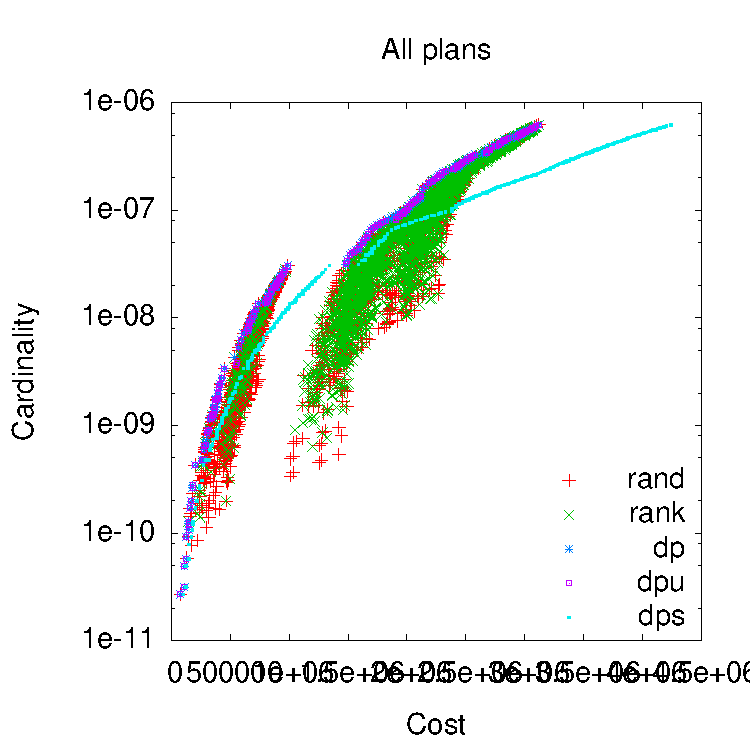
\includegraphics[width=0.49\linewidth]{figs/plans_q2_all.pdf}
  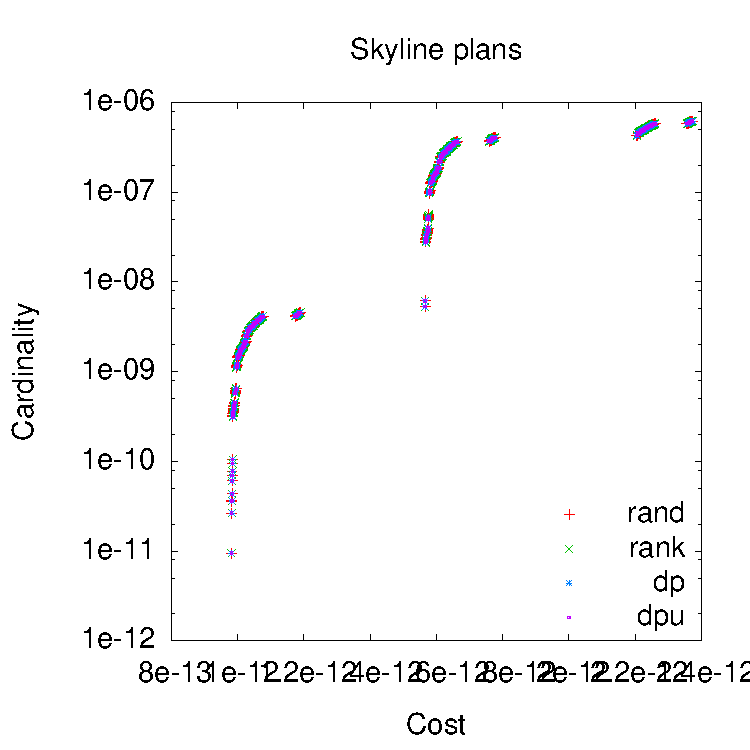
\includegraphics[width=0.49\linewidth]{figs/plans_q2_sky.pdf}
  \caption{Plans for query Q2 on all systems: a) all plans and b)
    skyline plans.}
  \label{fig:pareto_q2_skyline}
\end{figure}

\textbf{Execution Time.} \todo{execute several plans of some
  queries and show that execution time is better with fewer sources}

%%% Local Variables: 
%%% mode: latex
%%% TeX-master: "paper"
%%% End: 

\section{Conclusion}
\label{sec:conclusion}

We propose a first solution towards a systematic optimization of
Linked Data queries with an optimization framework for Linked Data
query processing, which incorporates both, standard query operators
and source selection. In order to support joint optimization of
multiple, conflicting objectives, such as cost and output cardinality,
we extend the classic dynamic programming solution for query
optimization to the multi-objective setting. The result is the Pareto
set of optimal query plans, representing the trade-off between the
optimization objectives. Further, we support sharing of source scan
operators and provide bounds on plan costs to ensure the optimality of
the dynamic programming algorithm. In experiments we compare our
solution to baselines and show that our approach improves on the
baselines by generating the complete Pareto set of optimal plans and
producing plans improve performance for the same number of results.

Future work lies in two main areas. The cardinality and cost
estimation of combinations of sources should be improved to take
dependencies between sources into account. The high complexity of the
multi-objective dynamic programming algorithm necessitates
investigation of approximative algorithms.

%%% Local Variables: 
%%% mode: latex
%%% TeX-master: "paper"
%%% End: 


\bibliographystyle{abbrv}
\bibliography{paper}

\begin{appendix}

\section{Appendix}
\label{sec:app}
\begin{figure}[htb]
  \centering
\begin{verbatim}
Q2
SELECT * WHERE {
  ?p dbowl:stateOfOrigin dbpedia:Italy .
  ?p owl:sameAs ?o .
  ?o a foaf:Person .
}
\end{verbatim}
 
\begin{verbatim}
Q5
SELECT * WHERE {
  ?n dcterms:subject dbpedia:Category:Western_Europe .
  ?n owl:sameAs ?p .
  ?p factbook:birthrate ?a .
}
\end{verbatim}

\begin{verbatim}
Q15
SELECT * WHERE {
  ?a dbowl:artist dbpedia:Michael_Jackson .
  ?a owl:sameAs ?a2 .
  ?a2 rdfs:label ?n .
}
\end{verbatim}

\begin{verbatim}
Q19
SELECT * WHERE {
  ?x dbprop:country dbpedia:Germany .
  ?x owl:sameAs ?o .
  ?o rdfs:label ?n
}
\end{verbatim}

  \caption{Queries Q2, Q5, Q15, and Q19}
\label{fig:qtp3}
\end{figure}


\begin{figure}[htb]
  \centering
\begin{verbatim}
Q1
SELECT * WHERE {
  ?x dcterms:subject dbpedia:Category:Liberal_democracies .
  ?x rdfs:label "Germany"@en .
  ?x owl:sameAs ?p .
  ?p rdfs:label ?n .
}
\end{verbatim}
 
\begin{verbatim}
Q3
SELECT * WHERE {
  ?n a dbowl:PopulatedPlace .
  ?n rdfs:label "Estonia"@en .
  ?n owl:sameAs ?a .
  ?a foaf:name ?t .
}
\end{verbatim}

\begin{verbatim}
Q4
SELECT * WHERE {
  ?drug drugbank:drugCategory drugcategory:micronutrient .
  ?drug drugbank:casRegistryNumber ?id .
  ?drug owl:sameAs ?s .
  ?s sider:sideEffect ?eff .
}
\end{verbatim}

\begin{verbatim}
Q6
SELECT * WHERE {
  ?n dcterms:subject dbpedia:Category:Chancellors_of_Germany .
  ?p owl:sameAs ?n .
  ?p nyt:first_use ?u .
  ?p nyt:topicPage ?page .
}
\end{verbatim}

\begin{verbatim}
Q7
SELECT * WHERE {
  mdb:director/8477 foaf:made ?film .
  ?film dcterms:date ?date .
  ?film foaf:page ?page .
  ?film owl:sameAs ?f2 .
}
\end{verbatim}

  \caption{Queries Q1, Q3, Q4, Q6, and Q7}
\label{fig:qtp4}
\end{figure}

\begin{figure}[htb]
  \centering
\begin{verbatim}
Q9
SELECT * WHERE {
  dailymed_orga:Mylan_Pharmaceuticals_Inc dailymed:producesDrug ?bd . 
  ?bd dailymed:genericDrug ?gd .
  ?gd drugbank:possibleDiseaseTarget ?dt . 
  ?dt owl:sameAs ?o .
  ?o rdfs:seeAlso ?n .
}
\end{verbatim}
 
\begin{verbatim}
Q14
SELECT * WHERE {
  ?a dbowl:artist dbpedia:The_Beatles .
  ?a rdfs:label "Yesterday"@de .
  ?a foaf:depiction ?img .
  ?b dbowl:previousWork ?a .
  ?b rdfs:label ?n .
}
\end{verbatim}

\begin{verbatim}
Q16
SELECT * WHERE {
  ?country a dbowl:Country .
  ?country rdfs:label "Monaco"@en .
  ?country owl:sameAs ?c2 .
  ?c2 factbook:unemploymentrate> ?n .
  ?c2 factbook:literacy_totalpopulation> ?l .
}
\end{verbatim}

\begin{verbatim}
Q17
SELECT * WHERE {
  ?film mdb:movie/actor mdb:actor/30064 .
  ?film mdb:movie/featured_film_location ?loc .
  ?loc rdfs:label "Hawaii (Film Location)" .
  ?film owl:sameAs ?f2 .
  ?f2 dbowl:music dbpedia:John_Williams .
}
\end{verbatim}

\begin{verbatim}
Q18
SELECT * WHERE {
  ?child geo-ont:parentFeature geonames:6269131 .
  ?child geo-ont:officialName "Cornwall" .
  ?child geo-ont:nearby ?n .
  ?n geo-ont:name ?nn .
  ?n a ?t .
}
\end{verbatim}

  \caption{Queries Q5, Q14, Q16, Q17, and Q18}
\label{fig:qtp5}
\end{figure}

%%% Local Variables: 
%%% mode: latex
%%% TeX-master: "paper"
%%% End: 
  
\end{appendix}
%%% Local Variables: 
%%% mode: latex
%%% TeX-master: "paper"
%%% End: 


\end{document}
